\documentclass[11pt]{article}

\usepackage[margin=1in]{geometry}
\usepackage{amsmath,amssymb,amsthm,mathtools}
\usepackage{enumitem}
\usepackage{array}
\usepackage{booktabs}
\usepackage{tikz}
\usetikzlibrary{positioning,arrows.meta,calc,backgrounds,fit}
\usepackage{hyperref}

\hypersetup{
  colorlinks=true,
  linkcolor=blue,
  citecolor=blue,
  urlcolor=blue
}

% --- Trellis / board figure styles ---
\tikzset{
  st/.style={circle, draw, thick, minimum size=8mm, inner sep=0pt, font=\footnotesize},
  goal/.style={circle, draw, thick, double, fill=yellow!55, minimum size=8mm,
               inner sep=0pt, font=\footnotesize},
  dead/.style={circle, draw, thick, fill=gray!12, minimum size=8mm,
               inner sep=0pt, font=\footnotesize, text=gray!60},
  lit/.style={line width=1.1pt, draw=blue!70!black, -{Stealth[length=2.2mm]}},
  alt/.style={draw=gray!70, dashed, -{Stealth[length=2.2mm]}},
  swlab/.style={font=\scriptsize, sloped, above=-1pt},
  swlabb/.style={font=\scriptsize, sloped, below=-1pt},
  col/.style={font=\small\bfseries},
}
\newtheorem{definition}{Definition}
\newtheorem{proposition}{Proposition}
\newtheorem{assumption}{Assumption}
\newtheorem{conjecture}{Conjecture}
\theoremstyle{remark}
\newtheorem{remark}{Remark}
\newtheorem{example}{Example}

\newcommand{\Effects}{\mathcal{E}}
\newcommand{\LTL}{\mathrm{LTL}}
\newcommand{\LTLf}{\mathrm{LTL}_f}
\newcommand{\AP}{\mathrm{AP}}
\newcommand{\Close}{\mathrm{Close}}
\newcommand{\Lang}{\mathcal{L}}
\newcommand{\Nat}{\mathbb{N}}
\newcommand{\True}{\mathsf{true}}
\newcommand{\Frame}{\mathfrak{F}}
\newcommand{\Design}{\eta}
\newcommand{\Adm}{\mathrm{Adm}}
\newcommand{\Lit}{\mathrm{Lit}}
\newcommand{\Causes}{\mathsf{Causes}}
\newcommand{\TRACE}{\textsc{Trace}}
\newcommand{\HOA}{\mathrm{HOA}}

\title{From Synthesized Controllers to a Playable Benchmark:\\
The Design of a Human- and AI-Playable Game for Temporal Causal Reasoning}
\author{}
\date{}

\begin{document}
\maketitle

\begin{abstract}
We turn a formal account of temporal causation into a benchmark of temporal
causal reasoning, grounded in TempoBench's temporal causal evaluation (TCE):
given a synthesized finite-state system, an observed trace, and an output ``$o$
at time $k$,'' name the timestep-indexed inputs that caused it. TempoBench
labels these with CORP, a tool in the Halpern--Pearl actual-causation tradition.
We frame TCE through three causal objects over the same device---count-only
\emph{necessity}, \emph{sufficiency}, and \emph{actual causation} (necessity
under a contingency)---and argue for actual causation as the core: we prove
that on input-deterministic, input-total controllers every minimal count-only
necessity cause is a \emph{singleton}, and that none exists exactly when no
single input flip destroys the effect (a verdict we call \emph{no pivotal
cell}). Count-only necessity therefore never returns a jointly-acting
multi-cell cause, and returns nothing at all on overdetermined effects, where
actual causation still has answers. Whether our actual-cause object equals the
per-cell key TempoBench derives from CORP is stated as an explicit conjecture.

We operationalize the construction as \TRACE{} (Temporal Reasoning And Causal
Explanation): a synthesized controller frozen into a one-player
switch-and-light device whose run flashes a target light. The player marks the
switches that decided the flash (\emph{Credit}) or plays the necessity
(\emph{Prevent}) and sufficiency (\emph{Pin}) readings; answers are scored by a
formal predicate that accepts any correct minimal cause, not a fixed string.
The same interface is exposed to AI agents as a JSON protocol with a budgeted
counterfactual probe and a verifiable reward. Humans and agents are graded on
identical information within each of two tracks: a \emph{white-box} track (the
machine shown; the primary reasoning track, matching TempoBench's information
setting) and a \emph{black-box} track (the machine hidden; system
identification plus causal reasoning, under an identifiability requirement).

\TRACE{} is ARC-AGI-\emph{inspired} in format---small, self-contained,
procedurally generable, verifiably graded---though it tests active temporal
credit assignment rather than ARC's static spatial induction. The paper closes
with a concrete validation-and-build roadmap: auditing the released TempoBench
artifacts against our assumptions (F1)--(F3), checking the CORP correspondence
on a sample, profiling the grader, and running human and agent baselines. An
appendix places the core at one corner of a lattice of richer variants, marking
where automatic scoring remains tractable.
\end{abstract}

\tableofcontents

\section{Introduction}
\label{sec:intro}

\subsection{The gap this benchmark targets}

ARC-AGI \emph{(Abstraction and Reasoning Corpus)} reopened a simple question:
can we build a task that is easy for humans, hard for machines, and resistant to
memorization, so that progress on it tracks reasoning rather than
recall~\cite{chollet2019measure}? Its puzzles are small grid transformations
specified by a handful of input/output examples; a solver must infer the rule
and apply it to a held-out input. ARC-AGI deliberately measures \emph{fluid}
intelligence---efficient acquisition of a new skill from little data---rather
than \emph{crystallized} knowledge, and it is calibrated so that its tasks
remain solvable by people while, at release, frontier models scored in the
single digits.\footnote{ARC-AGI-2 was released by the ARC Prize Foundation in
March 2025; its technical report is \cite{chollet2025arcagi2} (submitted May
2025, revised January 2026). The report describes removing
brute-force-solvable tasks and calibrating difficulty against timed human
panels, with every retained task solved by multiple human testers, while pure
language models scored near $0\%$ and public reasoning systems reached only
single-digit accuracy at release; current leaderboard figures may differ.}

ARC-AGI is spatial and abstraction-driven. It says little about a second kind of
reasoning that is central to programs, protocols, and agents: \emph{temporal
causal reasoning}---tracing, over a sequence of steps, which facts at or before
an event were \emph{necessary} for it. ``Why did the grant fire at step 7?''
``Which of the requests in the first five cycles actually mattered?'' These are
counterfactual questions about a temporal process, and they are exactly the kind
of credit-assignment reasoning that an agent acting over time must do.
TempoBench~\cite{holzer2025tempobench} introduced a formally grounded benchmark
in this space, built from reactive-synthesis artifacts, with two tasks:
\emph{temporal trace evaluation} (TTE), deciding whether a finite trace is
accepted by a supplied automaton, and \emph{temporal causal evaluation} (TCE),
asking which input facts caused a specified output at a specified timestep.
TempoBench phrases TCE as the inputs ``necessary'' for the output but computes
its answer key with CORP (``Causes for Omega-Regular Properties''), a cause
synthesis tool in the Halpern--Pearl actual-causation
tradition~\cite{finkbeiner2024corp,coenen2022temporal,halpernpearl2005causes};
we take that gap between the prose (necessity) and the method (actual
causation) seriously, because it determines what a ``correct answer'' is.

This paper does three things. First, it gives a self-contained, finite account of
TCE in terms of three causal objects---necessity, sufficiency, and actual
causation---argues that actual causation is the one that should match TempoBench's
labels (a checkable conjecture), and makes ``correct answer'' a formal predicate
rather than a
convention. Second, it separates TempoBench's production pipeline (which labels
causes with CORP) from \TRACE{}'s own generator, isolating exactly where a
ground-truth cause is computed and why it can be checked automatically. Third, it
translates the construction into a concrete game, played and graded on identical
information by humans and AI agents, and positions that game as a temporal-causal
analog of ARC-AGI.

\subsection{Why a formal cause makes a better benchmark}

A benchmark is only as good as its answer key. ARC grids are hand-authored and
graded by exact-output match; this is robust because the output is a single grid,
but it scales by human effort and admits only one accepted answer. Temporal
causal questions are different in two ways that the formal framework lets us
exploit:

\begin{itemize}[nosep]
  \item \textbf{Ground truth is computable.} For a point effect ``$o$ at time
        $k$,'' validity of a candidate cause is a finite, decidable check over the
        supplied automaton---a reachability query for sufficiency, a closest-removal
        or contingency search for necessity and actual cause---and minimality is a
        search over a finite (if exponential) space of input-constraint sets.
        Instances and their answer keys can be \emph{procedurally generated} from
        synthesized controllers, with difficulty tuned by observable features.
  \item \textbf{Correctness is set-valued, not string-valued.} Several
        incomparable minimal causes can exist for the same effect. A faithful
        grader therefore accepts \emph{any} formally valid, subset-minimal cause,
        scored by a checker, rather than penalizing a correct answer for
        differing from one canonical string. This is a more honest test of
        reasoning than exact match, and it is only available because we can
        \emph{decide} validity.
\end{itemize}

\subsection{Contributions}

\begin{enumerate}[label=(\arabic*)]
  \item \textbf{A finite account on three causal objects.} We restate the minimal
        framework and the TempoBench frame $\Frame_{\mathrm{TB}}$, and define
        \emph{necessity}, \emph{sufficiency}, and \emph{actual causation} finitely
        over the point effect $X^k o$ (Section~\ref{sec:framework}). We prove that
        count-only necessity collapses to singleton causes or the
        no-pivotal-cell verdict on input-deterministic, input-total controllers
        ((F2)--(F3); Proposition~\ref{prop:pivotal}), which is why
        \emph{actual causation}, not necessity, is the object aligned with
        TempoBench---an alignment we state as a checkable conjecture
        (Conjecture~\ref{conj:corp}), not a theorem.
  \item \textbf{The pipeline as a benchmark generator.} We trace the path
        SYNTCOMP/TLSF $\to$ LTLsynt $\to$ HOA $\to$ HOAX trace $\to$ effect $\to$
        cause, distinguishing TempoBench's CORP-labeled key from \TRACE{}'s own
        actual-cause generator, and analyzing its cost honestly
        (Section~\ref{sec:pipeline}).
  \item \textbf{\TRACE{}: a human-playable game design.} The frozen
        controller as a Turing-Tumble-style switch-and-light device; three
        one-player modes (\emph{Credit}/actual cause, \emph{Prevent}/necessity,
        \emph{Pin}/sufficiency); the budgeted counterfactual probe; predicate-based
        scoring at three granularities; difficulty knobs; and five fully worked
        puzzles (Section~\ref{sec:game}).
  \item \textbf{An information-parity AI-agent protocol.} A JSON
        observation/action interface matching the human game, with two tracks:
        a \emph{white-box} primary track that shows the machine to human and
        agent alike (TempoBench's information setting), and a \emph{black-box}
        track that hides it from both and adds a budgeted probe tool, subject
        to an identifiability requirement. Grading is a verifiable reward
        suitable for evaluation and RL, with a dated account of where the task
        is hard for current models (Section~\ref{sec:agent}).
  \item \textbf{The ARC-AGI analogy, made precise.} A point-by-point comparison
        and a statement of what \TRACE{} adds: decidable (predicate-checked)
        answers, procedural generation, and set-valued correctness
        (Section~\ref{sec:arc}).
  \item \textbf{A validation-and-build roadmap.} A concrete, ordered list of
        the steps that take the design to a released benchmark---artifact
        audit, CORP cross-check, grader implementation and profiling, corpus
        statistics, identifiability enforcement, and human/agent
        baselines---each stated as a falsifiable TODO
        (Section~\ref{sec:roadmap}).
  \item \textbf{A flexibility appendix.} Relaxing each TempoBench constraint axis
        yields a lattice of richer variants---bounded and liveness effects,
        output and strategy-structure interventions (the reverse parity game),
        profile-refined closeness, richer vocabularies, background assumptions,
        and the finite-to-infinite horizon step---with notes on which relaxations
        keep automatic scoring tractable and which do not
        (Appendix~\ref{app:flex}).
\end{enumerate}

\begin{center}
\fbox{\begin{minipage}{0.92\linewidth}
\textbf{Status of claims.}
\emph{Established here:} the definitions and propositions of
Section~\ref{sec:framework} (in particular the collapse of count-only
necessity, Proposition~\ref{prop:pivotal}), the grader predicates, and the game
and protocol design.
\emph{Conditional:} every TempoBench-equivalence claim, which rests on three
checkable artifact assumptions (F1)--(F3) and on Conjecture~\ref{conj:corp}
(that our actual-cause object equals the per-cell key TempoBench derives from
CORP).
\emph{Scheduled:} discharging (F1)--(F3) and Conjecture~\ref{conj:corp},
implementing and profiling the generator and grader, and human/agent
baselines are steps V1--V8 of the roadmap (Section~\ref{sec:roadmap}).
\end{minipage}}
\end{center}

\section{The Framework, Restated for This Paper}
\label{sec:framework}

This section is self-contained: it fixes the objects \TRACE{} needs without
assuming the companion documents. Readers familiar with the framework can skim to
Section~\ref{sec:tb-frame}.

\subsection{Systems, traces, and the supplied automaton}
\label{sec:systems}

A reactive system has disjoint input and output propositions $I$ and $O$
($I\cap O=\emptyset$). A complete valuation at one timestep is a set
$\alpha\subseteq I\cup O$; the input part is $\alpha\cap I$ and the output part is
$\alpha\cap O$. A \emph{finite trace} of length $n+1$ is
$\tau_{\le n}=\alpha_0\alpha_1\cdots\alpha_n$ with each
$\alpha_t\subseteq I\cup O$. An atom $p$ \emph{holds at} $t$ iff $p\in\alpha_t$;
the literal $\neg p$ holds iff $p\notin\alpha_t$. We write $\models$ for a trace
satisfying a temporal formula and read temporal operators over finite traces with
$\LTLf$ (finite-trace LTL) semantics~\cite{degiacomo2013ltlf}; the only operator
we need is the bounded next, with $X^k o$ true on $\tau_{\le n}$ iff
$o\in\alpha_k$ (defined whenever $k\le n$).

A synthesized controller is usually a Mealy machine
$M=(S,s_0,I,O,\delta,\lambda)$, $\delta:S\times 2^I\to S$,
$\lambda:S\times 2^I\to 2^O$. TempoBench, however, supplies the system as a
finite-state \emph{acceptor} rather than a transducer, serialized in the HOA
(Hanoi Omega-Automata) format~\cite{babiak2015hoa}, a standard text format for
$\omega$-automata in which transitions are labelled by Boolean formulas over
the atomic propositions.

\begin{definition}[Supplied automaton and admissibility]
\label{def:hoa}
$A_{\HOA}=(Q,2^{I\cup O},\delta,q_0,F)$ reads sequences of complete valuations.
TempoBench's TTE task uses final-state acceptance (run defined and
$q_{n+1}\in F$); for the \emph{behavior-set} role we need here, a finite trace
$\beta=\beta_0\cdots\beta_n$ is \emph{admissible} iff its run
$q_0\xrightarrow{\beta_0}q_1\cdots\xrightarrow{\beta_n}q_{n+1}$ is merely
\emph{defined} (every step exists). That is, we read the synthesized controller
as a safety/transducer object and do \emph{not} use $F$ to restrict behaviors
(equivalently, $F=Q$); $\Lang(A_{\HOA})$ is then ``the admissible behaviors of the
system,'' not an effect monitor, and $\Lang_{\le n}(A_{\HOA})$ is the admissible
(run-defined) sequences of length $n{+}1$. We use ``admissible'' in this
run-defined sense throughout (consistent with Section~\ref{sec:groundtruth}).
\end{definition}

\subsection{The causal frame}
\label{sec:frame}

The reverse-causal object is a \emph{frame}, which fixes everything an
explanatory question needs beyond the system itself:
\[
  \Frame=(B_{\Frame},E_{\Frame},S_{\Frame},O_{\Frame},
          \mathcal{K}_{\Frame},\mathcal{I}_{\Frame},{\preceq},\triangleleft).
\]
Here $B_{\Frame}$ is a background constraint (environment assumptions or held
guarantees; $\True$ if none); $E_{\Frame}$ is the effect to explain, possibly a
selected conjunct $\bigwedge_{r\in S_{\Frame}}E_r$ of a larger effect;
$O_{\Frame}\subseteq O$ the relevant outputs; $\mathcal{K}_{\Frame}$ the
candidate-cause space; $\mathcal{I}_{\Frame}$ the intervention model;
${\preceq}=\{\preceq_\tau\}$ the similarity orders on traces; and $\triangleleft$
a preference order on candidates ($C'\triangleleft C$: $C'$ is preferred). More 
simply: \emph{$M$ (or $A_{\HOA}$) gives behavior; $\Frame$ gives explanatory
scope.} A cause is always reported \emph{relative to} a declared frame.

The intervention model $\mathcal{I}_{\Frame}$ fixes the admissible counterfactual
set $\Adm_M^{\Frame}(\tau)$. The default and only regime needed for TempoBench is
\emph{input-only}: counterfactuals stay genuine behaviors and respect the
background, $\Adm_M^{\Frame}(\tau)=\Lang(M)\cap\Lang(B_{\Frame})$ (with
$\Lang(A_{\HOA})$ in place of $\Lang(M)$). Two further regimes---editing outputs,
or re-opening the controller's strategic commitments---are the subject of
Appendix~\ref{app:flex}.

\subsection{Closeness and valid causes}
\label{sec:causes}

Counterfactual necessity needs a notion of ``closest.'' Throughout, the unit of
change is an \emph{input cell}: a pair $(t,i)\in\{0,\ldots,n\}\times I$ recording
the value of one input proposition at one timestep. Because outputs are
determined by inputs (assumption (F2), Remark~\ref{rem:f1f2}), a counterfactual
is fixed by its input cells alone, and its outputs---including the effect---are
whatever the machine then produces. We therefore measure distance by the
\emph{chosen} input changes only, never by their determined output consequences
(otherwise flipping one early input, which the machine propagates to many later
outputs, would be counted as a large change). The canonical order is
\emph{count-only}: for the actual trace $\tau$, let
\[
  \mathrm{Diff}_\tau(\tau')=\bigl\{(t,i)\in\{0,\ldots,n\}\times I
     \;\big|\; [\,i\in\tau'(t)\,]\neq[\,i\in\tau(t)\,]\bigr\},
  \qquad d(\tau,\tau')=|\mathrm{Diff}_\tau(\tau')|,
\]
so fewer changed \emph{input cells} is closer. Under this count-only order the
closest removals form a \emph{set} (all minimum-count witnesses), and validity
quantifies over all of them. The closest admissible counterfactuals removing $C$
are
\[
  \Close_{\tau,M}^{\Frame}(\neg C)
  =\min\nolimits_{\preceq_\tau}
   \{\tau'\in\Adm_M^{\Frame}(\tau)\mid\tau'\models\neg C\}.
\]

\begin{definition}[Valid cause]
\label{def:valid}
$C\in\mathcal{K}_{\Frame}$ is a \emph{valid cause} of $E_{\Frame}$ on $\tau$ iff
all four clauses hold:
\begin{enumerate}[label=(\roman*),nosep]
  \item \textbf{Actuality:} $\tau\models C$ and $\tau\models E_{\Frame}$;
  \item \textbf{Non-vacuity:} $\Close_{\tau,M}^{\Frame}(\neg C)\neq\emptyset$
        (some admissible trace removes $C$);
  \item \textbf{Counterfactual dependence:}
        $\Close_{\tau,M}^{\Frame}(\neg C)\cap\Lang(E_{\Frame})=\emptyset$ (the
        effect fails on every closest removal);
  \item \textbf{Anti-circularity (syntactic):} $C$ does not name the effect atom
        at the effect position---for a point effect $X^k o$, no literal of $C$
        mentions $o$ at time $k$. A candidate may thus cause $E$ \emph{through}
        the machine but may not \emph{restate} it.
\end{enumerate}
$\Causes_{M,\Frame,\tau}(E_{\Frame})$ is the set of valid causes. A
\emph{minimal} cause $C^\star$ is a $\triangleleft$-minimal element; when
$\triangleleft$ is partial, several incomparable minimal causes may exist.
\end{definition}

Clause (ii) is what makes an answer non-trivial: a condition that no admissible
counterfactual can violate (a tautology, or an invariant of the system under
input-only intervention) is vacuous, not causal. Clause (iv) is a purely
\emph{syntactic} guard on the candidate. We deliberately do \emph{not} test the
semantic inclusion $\Lang(C)\subseteq\Lang(E_{\Frame})$: in a deterministic
system an input can entail the output \emph{precisely because it causes it}, so a
semantic test would wrongly reject genuine causes. Forbidding a candidate from
mentioning the effect atom at the effect position is enough to bar a ``cause''
that merely re-asserts the effect.

\subsection{The TempoBench frame}
\label{sec:tb-frame}

The TempoBench frame $\Frame_{\mathrm{TB}}$ fixes a deliberately simple setting:
\begin{itemize}[nosep]
  \item \textbf{Effect class:} a single positive output occurrence at a fixed
        timestep,
        $\mathcal{E}_{\mathrm{TB}}=\{X^k o\mid o\in O_{\Frame},\ 0\le k\le n,\
        o\in\alpha_k\}$. The selected effect is $E_{\Frame}=X^k o$.
  \item \textbf{Background:} $B_{\Frame}=\True$.
  \item \textbf{Intervention:} input-only; the automaton, outputs, transitions,
        and acceptance are not edited.
  \item \textbf{Candidate vocabulary:} timestep-indexed input literals over the
        causal window $0,\ldots,k$. Here a \emph{literal} $\ell\in\Lit(I)$ is an
        input proposition or its negation,
        $\Lit(I)=\{i,\neg i\mid i\in I\}$, and a pair $(t,\ell)$ reads ``literal
        $\ell$ is required at timestep $t$.'' A candidate is then a constraint set
        $\Gamma\subseteq\{0,\ldots,k\}\times\Lit(I)$, denoting the bounded formula
        $C_\Gamma=\bigwedge_{(t,\ell)\in\Gamma}X^t\ell$. There are at most
        $2|I|(k{+}1)$ literals, hence
        $|\mathcal{K}_{\Frame_{\mathrm{TB}}}|\le 2^{2|I|(k+1)}$ constraint
        sets---finite but exponential in the window. (A set containing both $i$
        and $\neg i$ at one timestep is contradictory and fails actuality; since
        exactly one literal per input cell holds on the fixed actual trace, the
        candidates that can pass actuality number at most $2^{|I|(k+1)}$.)
  \item \textbf{Closeness:} the count-only coarsening (fewer changed input cells
        is closer); $\Close$ is the full minimum-count set.
  \item \textbf{Preference:} subset minimality on $\Gamma$ (not formula size or
        automaton size).
\end{itemize}

\paragraph{Finite valid causes.} A counterfactual is itself a finite trace
$\beta=\beta_0\cdots\beta_n$ (a valuation sequence of the same length as
$\tau_{\le n}$, with each $\beta_t\subseteq I\cup O$ and $\beta_k$ its valuation at
the effect position); it is \emph{admissible} when accepted by $A_{\HOA}$, i.e.\
$\beta\in\Adm^{\le k}_{A}=\Lang_{\le n}(A_{\HOA})$. A \emph{removal} for $\Gamma$ is
an admissible $\beta$ that violates $C_\Gamma$ (it changes at least one required
input literal). With the change-counting order,
\[
  \Close^{\le k}_{\tau_{\le n},A}(\neg C_\Gamma)
  =\min\nolimits_{\#\text{changes}}
   \{\beta\in\Adm^{\le k}_{A}\mid\beta\not\models C_\Gamma\},
\]
\[
\begin{aligned}
  \Causes^{\le n}_{A,\Frame_{\mathrm{TB}},k}(X^k o)=\{\Gamma\mid{}&
  \tau_{\le n}\models C_\Gamma,\ o\in\alpha_k,\
  \Close^{\le k}_{\tau_{\le n},A}(\neg C_\Gamma)\neq\emptyset,\\
  &\forall\beta\in\Close^{\le k}_{\tau_{\le n},A}(\neg C_\Gamma).\ o\notin\beta_k\}.
\end{aligned}
\]
A minimal cause $C^\star=C_{\Gamma^\star}$ uses any subset-minimal valid
$\Gamma^\star$ (several may exist). Anti-circularity (clause (iv)) is automatic
here: candidates are input literals and the effect is an output occurrence, so a
candidate never names the effect atom at the effect position.

\subsection{The reduction, and its two assumptions}
\label{sec:reduction}

\begin{remark}[What $A_{\HOA}$ must be]
\label{rem:f1f2}
The finite construction models the supplied automaton as the system's behavior
set, which requires two assumptions, both checkable against the artifacts.
\textbf{(F1) Behavior model:} $\Lang(A_{\HOA})$ is exactly the set of system
executions, not a specification monitor $A_\varphi$ whose language is the
specification-satisfying traces. \textbf{(F2) Functionality:} the behavior set is
functional in the inputs (input-deterministic), so each input sequence has at most
one accepted $I\cup O$ completion---consistent with TempoBench's automata coming
from reactive synthesis, and exactly what lets us speak of ``the'' output at each
timestep. Both are mechanically checked by an audit in the verification suite
accompanying this repository (\texttt{Verification/}), validated against
labelled positive and negative controls: automata with nondeterministic output
completions, nondeterministic successors, undefined input valuations, and a
specification monitor are all classified correctly, for labels given over AP
indices and over AP names. The one publicly available TempoBench artifact (the
six-state arbiter embedded in the released tool) satisfies (F1)'s operational
conditions, (F2), and (F3); corpus-wide rates await the dataset's re-release
(it was withdrawn from distribution for re-preparation). The alignment remains
conditional only for artifacts not yet audited: if (F1) fails because a
supplied automaton is a specification monitor, the construction does not apply
to that artifact, and the audit detects this case.
\end{remark}

\begin{proposition}[Finite specialization---a definitional correspondence]
\label{prop:tb-reduction}
Assume (F1)--(F2). With $\Frame_{\mathrm{TB}}$ as the input-only frame,
$B_{\Frame}=\True$, admissible set $\Lang_{\le n}(A_{\HOA})$, the change-counting
order, and subset minimality, and interpreting the general clauses of
Definition~\ref{def:valid} over finite traces with $\LTLf$ semantics: for every
$\Gamma$, $\Gamma\in\Causes^{\le n}_{A,\Frame_{\mathrm{TB}},k}(X^k o)$ iff
$C_\Gamma$ satisfies the four valid-cause clauses on $\tau_{\le n}$ under
$\Frame_{\mathrm{TB}}$. The finite construction \emph{is} the general definition
restricted to a point effect; no infinitary acceptance for $A_{\HOA}$ is used.
\end{proposition}

This is a definitional restatement, not a deep theorem: each clause refers only
to positions $0,\ldots,k$, so it is a statement about length-$(k{+}1)$ prefixes
under $\LTLf$. It pins down precisely what our count-only \emph{necessity}
object is; whether that object coincides with TempoBench's TCE labels is a
separate, semantic question taken up in Section~\ref{sec:two-questions}, where
count-only necessity turns out to be the wrong object for them.

\begin{remark}[Validity is not monotone]
\label{rem:nonmonotone}
Membership in $\Causes^{\le n}$ is not monotone under $\subseteq$ on $\Gamma$:
enlarging $\Gamma$ can make a candidate valid (the cheapest removal must now flip
more) or invalid (the closest removal flips an irrelevant added literal while
keeping the output). So ``delete literals while valid'' need not reach a
subset-minimal cause; computing a minimal cause needs genuine search. Each
validity check is polynomial (finite reachability over $A_{\HOA}$ on the window);
the search is the hard part. This non-monotonicity is also what makes the game
non-trivial for a human or agent: there is no safe greedy shortcut.
\end{remark}

\subsection{Three causal objects, and what TempoBench computes}
\label{sec:two-questions}

``Which inputs mattered for that flash?'' has more than one precise reading, and
the readings genuinely disagree. We make three explicit---\emph{necessity},
\emph{sufficiency}, and \emph{actual causation}---show how they relate, and
identify which one TempoBench's TCE labels compute. The game of
Section~\ref{sec:game} exposes all three as one-player tasks over the same
device.

\paragraph{Why count-only necessity alone is not enough.} The valid-cause object
of Definition~\ref{def:valid} is the strictest reading: an input cell matters
only if, among the \emph{fewest} possible changes, altering it already destroys
the effect. Synthesized controllers are \emph{typically} input-total, which we
make explicit as a checkable assumption.

\begin{assumption}[Input-totality, (F3)]
\label{ass:input-total}
Every input sequence over $0,\ldots,n$ extends to an admissible (run-defined)
trace of $A_{\HOA}$; in particular, flipping any one input cell of $\tau_{\le n}$
again yields an admissible trace. Like (F1)--(F2), this is mechanically
checked by the audit described in Remark~\ref{rem:f1f2}; the available
TempoBench sample artifact satisfies it.
\end{assumption}

\begin{proposition}[Count-only necessity collapses to single pivotal inputs]
\label{prop:pivotal}
Assume $\Frame_{\mathrm{TB}}$ with count-only closeness, (F2), and (F3). Then every
subset-minimal valid cause is a \emph{singleton}: either some single input-cell
flip falsifies $X^k o$---and each such cell $\{(t,\ell)\}$ is a minimal cause---or
no single flip does, in which case $\Causes^{\le n}=\emptyset$. We call the
latter outcome the \emph{no-pivotal-cell} verdict: no literal-conjunction valid
cause exists.
\end{proposition}

\begin{proof}
To violate $C_\Gamma=\bigwedge_{(t,\ell)\in\Gamma}X^t\ell$ it suffices to falsify
one conjunct, and flipping that one input cell yields, by (F3), an admissible trace
that is, by (F2), \emph{unique}; so this is an admissible $1$-change removal, the
minimum change count is $1$, and $\Close^{\le k}(\neg C_\Gamma)$ is exactly the set
of single flips of $\Gamma$'s literals. If $\Gamma$ is valid, every such flip
falsifies $X^k o$; pick any $(t_0,\ell_0)\in\Gamma$ and note its single flip is the
unique closest removal of $\{(t_0,\ell_0)\}$ and falsifies the effect, so
$\{(t_0,\ell_0)\}$ is itself valid. Hence no valid $\Gamma$ with $|\Gamma|\ge 2$ is
subset-minimal. If instead no single flip falsifies $X^k o$, then no singleton is
valid and (by the same argument) neither is any larger set, so
$\Causes^{\le n}=\emptyset$.
\end{proof}

Two clarifications sharpen the proposition. First, the collapse concerns the
\emph{shape of each minimal cause}, not the per-cell union: several distinct
singleton pivots may coexist (Puzzle~4 has two), so the union of necessity
causes can still span multiple cells. What count-only necessity can
\emph{never} return, under (F2)--(F3), is a jointly-acting multi-cell cause (a
minimal cause of size $\ge 2$). Second, the no-pivotal-cell verdict is itself
ambiguous between two situations that the actual-cause object distinguishes:
the effect may be \emph{overdetermined}---no single flip suffices but actual
causes exist under a contingency (Puzzles~3 and~5)---or it may be
\emph{input-unconditional on the window}---no combination of in-window input
changes destroys it, in which case nothing is a cause under any of our
readings, and the instance is discarded by the trivial-instance filter of
Section~\ref{sec:difficulty}. Count-only necessity thus diverges from a
Halpern--Pearl key exactly on overdetermined and jointly-overdetermining
structure; on a prototype corpus of randomly generated input-deterministic,
input-total transducers, 11 of 139 generated instances were overdetermined
no-pivotal-cell cases (a further 4 were input-unconditional and discarded),
and the original-versus-modified variant keys diverged on 59\% of retained
instances---so the divergence class is common, not exotic; the corresponding
frequencies on TempoBench's own corpus await its re-release, and any nonempty
key on an overdetermined instance already separates the two objects. This collapse of strict counterfactual dependence
under overdetermination is exactly the phenomenon Halpern and Pearl introduced
contingencies to handle~\cite{halpernpearl2005causes}; our part is to make it
precise for synthesized temporal controllers and to build on the reading that
survives it.

\paragraph{What TempoBench's key generator computes: a form of actual
causation.} TempoBench computes its TCE answer key with
\emph{CORP}~\cite{finkbeiner2024corp}: Algorithm~1 of the TempoBench paper
invokes \texttt{corp} on the automaton, trace, and
effect~\cite{holzer2025tempobench}. CORP synthesizes $\omega$-regular causes
for $\omega$-regular effects, generalizing the \emph{temporal causality} of
Coenen et al.~\cite{coenen2022temporal}, a counterfactual, closest-trace
account that its authors place in the actual-causation tradition of Halpern and
Pearl~\cite{halpernpearl2005causes}; CORP's causes are themselves
$\omega$-regular automata, which may express disjunctions and temporal
patterns, not merely conjunctions of literals. The Halpern--Pearl tradition's
defining move is the \emph{contingency}: a cause must toggle the effect under
\emph{some} held-fixed setting of the other variables---not necessarily their
actual setting---while, with the cause in place, the effect still obtains
under that setting. Permitting a \emph{non-actual} contingency is exactly what
count-only closeness forbids, and it is what lets actual causation return
answers without the collapse of Proposition~\ref{prop:pivotal}. We now give
the sufficiency and actual-cause objects finitely.

\begin{definition}[Sufficient set / determining set]
\label{def:determining}
Fix $A_{\HOA}$, $\tau_{\le n}$, and a point effect $X^k o$ with $o\in\alpha_k$. A
set $\Gamma\subseteq\{0,\ldots,k\}\times\Lit(I)$ with $\tau_{\le n}\models C_\Gamma$
is \emph{sufficient} (it \emph{pins} the effect) iff every admissible
$\beta\in\Lang_{\le n}(A_{\HOA})$ with $\beta\models C_\Gamma$ has $o\in\beta_k$:
fixing the inputs named by $\Gamma$ to their actual values forces the output at
$k$ regardless of the other inputs. A \emph{determining set} is a subset-minimal
sufficient $\Gamma$. Sufficiency is decided by a finite non-emptiness check
(``is there an admissible $\beta\models C_\Gamma$ with $o\notin\beta_k$?'');
several incomparable determining sets may exist.
\end{definition}

\begin{definition}[Actual cause; finite Halpern--Pearl, with non-actual
contingencies]
\label{def:actual}
Fix $A_{\HOA}$, $\tau_{\le n}$, and a point effect $X^k o$ with $o\in\alpha_k$. A
\emph{contingency} assigns (possibly non-actual) values $w$ to a set
$W\subseteq\{0,\ldots,k\}\times I$ of in-window input cells. Under (F2)--(F3) each
input assignment determines a unique admissible trace; write
$\beta\langle W{=}w,\ \Gamma{=}v\rangle$ for the admissible trace with $W$ set to
$w$, the cells of $\Gamma$ set to $v$, and every other in-window cell at its
actual value. A nonempty $\Gamma\subseteq\{0,\ldots,k\}\times\Lit(I)$ (its
literals at their actual values, disjoint from $W$) is an \emph{actual cause} of
$X^k o$ iff:
\begin{description}[leftmargin=1.5cm,style=nextline,nosep]
  \item[\textnormal{(AC1)}] \emph{actuality:} $\tau_{\le n}\models C_\Gamma$ and
        $o\in\alpha_k$;
  \item[\textnormal{(AC2)}] \emph{contingency:} for some $(W,w)$, both
        \emph{(a, necessity)}
        $o\notin\beta\langle W{=}w,\ \Gamma{=}\overline{\mathrm{act}}\rangle_k$
        (with $W$ at $w$, flipping $\Gamma$ off its actual values destroys the
        effect) and \emph{(b, sufficiency)} for \emph{every} subset
        $W'\subseteq W$,
        $o\in\beta\langle (W{\setminus}W'){=}w,\ W'{=}\mathrm{act},\
        \Gamma{=}\mathrm{act}\rangle_k$ (with $\Gamma$ in place the effect
        survives the contingency, and survives \emph{robustly}: resetting any
        subset of the contingency cells to their actual values cannot destroy
        it; $W'=\emptyset$ recovers the plain case);
  \item[\textnormal{(AC3)}] \emph{minimality:} no proper subset of $\Gamma$
        satisfies AC1--AC2.
\end{description}
The sufficiency leg AC2(b) is what separates actual causation from bare
counterfactual dependence: without it, a contingency that suppresses the effect on
its own would spuriously license any candidate. On a \emph{singleton} candidate,
AC2(a) with $W=\emptyset$ is exactly count-only counterfactual dependence
(Definition~\ref{def:valid}); and since under (F2)--(F3) every count-only valid
cause is a singleton (Proposition~\ref{prop:pivotal}), the necessity \emph{object}
is the empty-contingency, singleton case of actual causation. (For a multi-cell
candidate the two notions of ``removal'' differ---closest violation vs.\ flipping
the whole candidate---so we make the special-case claim only for singletons.) The
\emph{actual-cause set} $\Gamma^{\mathrm{ac}}$ is the union of all (subset-minimal)
actual causes---a \emph{set of cells}, not itself a single cause; several
incomparable actual causes may exist.
\end{definition}

\paragraph{Why this is Halpern--Pearl, and which Halpern--Pearl.} The trellis is
a structural causal model: the in-window input cells are the exogenous variables,
the controller's deterministic transition-and-output map (under (F2)) is the
system of structural equations, and $o$ at $k$ is the endogenous effect.
AC1/AC2(a)/AC2(b)/AC3 instantiate the Halpern--Pearl conditions on this model in
the \emph{original/updated} variant~\cite{halpernpearl2005causes}, in which the
contingency cells $W$ may be held at \emph{non-actual} values. This is not
Halpern's later \emph{modified} definition~\cite{halpern2015modification},
which restricts $W$ to its actual values; the choice matters exactly on
overdetermined instances---under the modified definition Puzzle~3's cause would
be the joint pair $\{(0,a),(0,b)\}$, not the two singletons we report.
We have checked the contingency discipline of CORP's underlying definition
against the primary sources, and it does \emph{not} match ours. Coenen et
al.~\cite{coenen2022temporal} adopt actual causality ``in the version modified
by Halpern,'' and their contingency mechanism resets \emph{outputs} to the
values they take on the actual trace (``jumps'' back to $\tau$); the CORP tool
paper states the mechanism is ``inspired by Halpern's modified version of
actual causality'' and exposes contingencies as a toggle in implementations.
Definition~\ref{def:actual}'s contingencies---\emph{input} cells at possibly
\emph{non-actual} values---therefore follow a different discipline, so
Conjecture~\ref{conj:corp} cannot be discharged definitionally; if it holds
at all, it holds at the per-cell granularity, and symmetric overdetermination
is the predicted divergence class (under the modified discipline, Puzzle~3's
key is the joint pair rather than the two singletons).
Independent of CORP, the variant choice is deliberate: a credit-assignment
benchmark should attribute credit under symmetric overdetermination (Puzzle~3's
``each switch is a cause'' verdict matches the intuitive answer and is the one
TempoBench-style per-cell keys can express), whereas the modified definition's
joint answer cannot distinguish two independently sufficient switches from two
switches that act only jointly (Puzzle~4)---a distinction the game is built to
probe. Because every candidate cell here is exogenous, the usual HP subtlety
of partitioning endogenous variables into held-fixed ($W$) and floating ($Z$)
sets largely collapses, and the definition admits a plain restatement:
\emph{$\Gamma$ is an actual cause iff there is a setting of the other input
cells under which flipping $\Gamma$ off its actual values destroys the effect
while $\Gamma$ at its actual values (robustly) preserves it.} We do \emph{not}
prove that this finite, literal-cell object coincides with CORP's
$\omega$-regular construction---that is Conjecture~\ref{conj:corp}. Absent it,
Definition~\ref{def:actual} is best read as \emph{trellis actual causation}:
HP-style, but defined here.

\paragraph{How the three relate.}
\begin{itemize}[nosep]
  \item \textbf{Count-only necessity} (Def.~\ref{def:valid}) is actual causation
        with the \emph{empty} contingency on the \emph{singleton} candidates it
        admits (Proposition~\ref{prop:pivotal})---strictest and cheapest, kept as a
        deliberately strict diagnostic (the \emph{Prevent} mode).
  \item \textbf{Sufficiency} (Def.~\ref{def:determining}) is its \emph{dual}, not a
        special case: a set that \emph{forces} the effect over \emph{all} admissible
        inputs (the \emph{Pin} mode). This \emph{global} sufficiency is the
        unconditional analog of AC2(b)'s \emph{local} sufficiency (under a fixed
        contingency $W$)---related, but not the same object.
  \item \textbf{Actual causation} (Def.~\ref{def:actual}) combines a necessity leg
        (AC2(a)) and a local-sufficiency leg (AC2(b)) under a shared contingency, so
        an actual cause is, informally, a counterfactually necessary part of a
        locally sufficient set---a characterization standard in the Halpern--Pearl
        literature that we use as intuition, not a theorem. This is the core object
        \TRACE{} grades against, and the one we \emph{hypothesize} matches
        TempoBench's labels (Conjecture~\ref{conj:corp}).
\end{itemize}
On Puzzle~3 below (effect fires if $a$ \emph{or} $b$ is set, both set) count-only
necessity reports no pivotal cell, whereas actual causation returns both
$\{(0,a)\}$ and $\{(0,b)\}$ (hold the other off; each is then pivotal and, alone,
sufficient). A caution about evidence: at the per-cell granularity TempoBench
grades, \emph{Credit} and \emph{Pin} often \emph{agree}---on every worked puzzle of
Section~\ref{sec:worked} the actual-cause set equals the union of determining sets,
and only \emph{Prevent} differs by collapsing. Whether that per-cell equality
holds in general on (F2)--(F3) instances is open---though on a prototype
corpus of 107 randomly generated input-deterministic, input-total transducers
the per-cell equality held on \emph{every} instance at exhaustive search
depth, strengthening the case that a proof exists. (The same experiment
yielded a methodological caution: with the minimal-cause search capped at
three cells, 49 spurious divergences appeared; key searches must be exhaustive
or carry per-instance certificates.) A proof would make the
per-cell conjecture independent of the \emph{Credit}-vs-\emph{Pin} choice, and a
counterexample would be exactly the instance that justifies \emph{Credit}
specifically. So the case for actual causation as
the core is not that it out-predicts sufficiency cell-by-cell here; it is
\emph{definitional lineage}---CORP implements Halpern--Pearl temporal causality
(necessity-under-contingency \emph{and} sufficiency), not pure sufficiency
synthesis, so neither half alone is its object. Where the readings genuinely
diverge is in how cells group into minimal causes (the witness and all-causes
granularities, Section~\ref{sec:scoring}), not in the per-cell union.

\begin{conjecture}[Correspondence to CORP, at per-cell granularity]
\label{conj:corp}
For TempoBench instances satisfying (F1)--(F3),
$\Gamma^{\mathrm{ac}}$ (Definition~\ref{def:actual}) equals the timestep-indexed
cell set of TempoBench's shipped TCE answer key---i.e.\ TempoBench's own
per-cell rendering of CORP's output---for the same trace and effect. We state
this as a \emph{conjecture}. CORP's causes are $\omega$-regular automata and may
be disjunctive or temporally structured, whereas $\Gamma^{\mathrm{ac}}$ is a set
of literal cells; rather than define our own flattening of an $\omega$-regular
cause to cells, we anchor the comparison on the per-cell key TempoBench itself
derives and grades against, which makes the conjecture checkable against an
observable artifact. What we establish unconditionally is structural: \TRACE{}
computes a Halpern--Pearl actual-causation object over the same synthesized
device. Current evidence: an independent reference implementation of
$\Gamma^{\mathrm{ac}}$ (in the repository's verification suite) matches the
per-cell answer key of the one publicly available TempoBench TCE instance
exactly (and identically under the modified-variant reading, since that
instance is not overdetermined); the five worked puzzles of
Section~\ref{sec:worked} are likewise reproduced mechanically from HOA
encodings. Corpus-scale comparison awaits the dataset's re-release; given the
contingency-discipline mismatch established above, we expect agreement on
non-overdetermined instances and predict divergence---or the need to restate
the conjecture under the modified discipline---exactly on overdetermined
ones.
\end{conjecture}

\paragraph{Variant policy (adopting the verification suite's decision record).}
The discipline mismatch forces a policy, and we state it rather than let one
object play two roles. A benchmark corpus declares exactly \emph{one}
Halpern--Pearl variant per instance file. Corpora whose purpose is
\emph{TempoBench alignment} grade in the \emph{modified} discipline---CORP's
own---so that any alignment claim, if it survives the corpus-scale comparison,
is stated in the variant the compared tool actually implements. Corpora
advancing this paper's \emph{credit-assignment} argument grade in the
original/updated variant of Definition~\ref{def:actual}, which we keep as the
core for the reasons argued above (per-cell credit under symmetric
overdetermination)---an \emph{independent} stance, not an equivalence stance.
Instances on which the two variants disagree carry an \texttt{overdetermined}
difficulty tag. In the playable \emph{Credit} mode the variant is not named
but \emph{shown}: the win gesture is the player's own exhibited
contingency pair of runs, which is precisely the original/updated object, so
the play surface and the declared-variant grading cannot drift apart.

\section{A Benchmark Generator for the TCE Setting}
\label{sec:pipeline}

A benchmark needs three things: instances, answer keys, and a grader. We trace a
pipeline that produces all three, from specification to certified cause. The
front end---specification, synthesis, trace generation---is shared with
TempoBench, which builds instances from SYNTCOMP/TLSF specifications synthesized
by LTLsynt and drives them with the trace generator
HOAX~\cite{holzer2025tempobench}. The back end is where \TRACE{} and TempoBench
differ at the key step: TempoBench labels causes with CORP, whereas \TRACE{}
computes the actual-cause object of Definition~\ref{def:actual} by its own
search; the two are conjectured to agree (Conjecture~\ref{conj:corp}).
Throughout, ``the solver'' is whoever answers the TCE question---a person, an
agent, or our own ground-truth procedure.

\paragraph{Why an own grader rather than CORP as oracle.} Three reasons, none
of them a judgment on CORP. First, grading requires a \emph{per-candidate
predicate}: the checker must decide validity and minimality of any constraint
set a player submits, whereas CORP \emph{synthesizes} one $\omega$-regular
cause automaton per query---it is a generator, not a membership oracle at the
literal-cell granularity \TRACE{} grades. Second, the finite-window,
literal-cell objects of Section~\ref{sec:framework} feed the JSON protocol and
the subset-minimality certificates directly, with no flattening step inside
the grading loop. Third, keeping the key computation independent turns the
CORP comparison (roadmap step~V2) into a genuine cross-validation of both
implementations rather than a self-check.

\subsection{Production path}
\label{sec:production}

\begin{enumerate}[label=\textbf{P\arabic*.},leftmargin=2.4em]
  \item \textbf{Specification.} Take a reactive-system specification from a
        standardized corpus. TempoBench draws on the SYNTCOMP benchmark
        suite~\cite{jacobs2024syntcomp}, expressed in
        TLSF~\cite{jacobs2016tlsf}, which cleanly separates inputs, outputs,
        and their temporal behavior. A specification is an LTL (or TLSF)
        contract $\varphi$ over $I\cup O$.
  \item \textbf{Synthesis.} Synthesize a controller realizing $\varphi$ with a
        reactive-synthesis tool (ltlsynt from
        Spot~\cite{renkin2023ltlsynt}), producing an implementation in HOA
        format~\cite{babiak2015hoa} that preserves the input/output partition.
        This is the artifact $A_{\HOA}$ of Definition~\ref{def:hoa}; by
        construction it is an implementation, which is what makes assumptions
        (F1)--(F2) plausible (Remark~\ref{rem:f1f2}).
  \item \textbf{Trace generation.} Drive $A_{\HOA}$ with an input sequence to
        produce a finite observed trace $\tau_{\le n}=\alpha_0\cdots\alpha_n$ over
        $I\cup O$ (this is what TempoBench's HOAX~\cite{distefano2025hoax} does).
        Trace length $n$ is a difficulty knob.
  \item \textbf{Effect selection.} Choose a target output occurrence: pick
        $o\in O_{\Frame}$ and a timestep $k\le n$ with $o\in\alpha_k$, giving the
        point effect $E_{\Frame}=X^k o$. The causal window is $0,\ldots,k$; later
        timesteps are irrelevant to a point effect at $k$.
  \item \textbf{Ground-truth cause.} This is the step that is ours, not
        TempoBench's: where TempoBench calls CORP, \TRACE{} computes the
        actual-cause object of Definition~\ref{def:actual} for $X^k o$ under
        $\Frame_{\mathrm{TB}}$ (the actual-cause set $\Gamma^{\mathrm{ac}}$ and
        its minimal witnesses; Section~\ref{sec:groundtruth}). Under
        Conjecture~\ref{conj:corp} the two keys coincide on instances
        satisfying (F1)--(F3); the key the grader certifies is \TRACE{}'s
        actual-cause object.
  \item \textbf{Packaging.} Emit the instance---$A_{\HOA}$, the AP list, the trace
        $\tau_{\le n}$, and the effect $X^k o$---together with the hidden key
        $\Gamma^\star$ (or, better, the validity oracle itself; see
        Section~\ref{sec:groundtruth}).
\end{enumerate}

The solver is given P1's outputs through P4 (the AP list, $\tau_{\le n}$, and
$X^k o$, plus $A_{\HOA}$ in the white-box track); it is \emph{not} given $\varphi$,
the synthesis trace, or any internal structure beyond the automaton. The two
\TRACE{} tracks differ exactly here: the \emph{white-box} track (the primary
reasoning track) exposes $A_{\HOA}$---the information setting that matches
TempoBench's TCE, where the solver is handed the machine---while the
\emph{black-box} track withholds it and the solver recovers behavior through
the probe tool (Section~\ref{sec:agent}). In neither case
is the solver asked to synthesize a controller, choose a trace or effect, or recover
$\varphi$: it performs finite-horizon causal credit assignment over a provided
execution. TempoBench's reported scores bear on the white-box (machine-given)
setting, not the black-box one.

\subsection{Computing and certifying the answer key}
\label{sec:groundtruth}

The whole benchmark rests on step P5, so we make it precise.

\paragraph{What the automaton means.} We read $A_{\HOA}$ as an explicitly
represented, transducer-style \emph{behavior set}, not an effect monitor: a
finite valuation sequence $\beta_{\le n}$ is \emph{admissible} iff it labels a
run from $q_0$ whose every step is defined. Under (F2) each input sequence has
exactly one admissible $I\cup O$ completion, so ``the output at $k$'' is well
defined and a counterfactual is fully specified by its input cells on
$0,\ldots,n$. We do not rely on a final-state acceptance condition: the prefixes
we test are the admissible ones, and for a point effect $X^k o$ only the prefix
$0,\ldots,k$ is relevant, because the output at $k$ depends only on inputs
through $k$ (the causal, Mealy reading; later inputs cannot reach back).

\paragraph{Validity is a finite check.} Fix a candidate $\Gamma$. Actuality is
read directly off $\tau_{\le n}$ ($\tau_{\le n}\models C_\Gamma$ and
$o\in\alpha_k$). For counterfactual dependence we (a) find the minimum number $m$
of changed \emph{input cells} that yields an admissible trace violating
$C_\Gamma$, and (b) confirm that \emph{every} such minimum-change admissible
removal has $o\notin\beta_k$. Concretely, build the product of $A_{\HOA}$ with a
small monitor that (i) enforces $\neg C_\Gamma$, (ii) tracks the number of input
cells changed relative to $\tau_{\le n}$, and (iii) records whether $o$ holds at
$k$; a breadth-first search over change count returns the closest removals and
their effect status. Under (F2) the question ``does an admissible completion with
these inputs put $o$ at $k$?'' coincides with ``simulate these inputs and read off
$o$ at $k$.''

\paragraph{What a validity check costs.} We state bounds rather than a blanket
``polynomial.'' A caution first: HOA files store transition labels
\emph{symbolically}, as Boolean formulas over the atomic
propositions~\cite{babiak2015hoa}, so the explicit transition graph must be
obtained by a one-time expansion that is exponential in $|I|$ ($O(|Q|\cdot
2^{|I|})$ edges). All bounds below are stated against that \emph{expanded}
graph: $|A_{\HOA}|$ denotes the explicit size---states \emph{and}
input-labelled transitions, the latter already $O(|Q|\cdot 2^{|I|})$---and the
expansion cost is paid once per instance, kept tractable by capping $|I|$ (a
difficulty knob). Stated against the symbolic description instead, none of the
polynomial claims below survive. Simulating one fixed input sequence is linear in
$|A_{\HOA}|$ and $k$. \emph{Sufficiency} (Definition~\ref{def:determining}) is a
reachability/non-emptiness query over the product---``can any admissible
completion consistent with $\Gamma$ avoid $o$ at $k$?''---hence polynomial in
$|A_{\HOA}|$ and $k$. \emph{Closest-removal necessity} (Definition~\ref{def:valid})
is a minimum-Hamming shortest-path search over the same explicit product (states
$\times$ window position $\times$ change count); because the $2^{|I|}$ edge
fan-out is \emph{already} counted in $|A_{\HOA}|$, this too is polynomial in
$|A_{\HOA}|$, $k$, and $|I|$, not separately exponential. The genuine blow-up is
\emph{actual causation} (Definition~\ref{def:actual}), which wraps the necessity
check in an outer search over contingencies $(W,w)$. With $N=|I|(k{+}1)$ binary
in-window cells, a contingency is a partial assignment---each cell is
unconstrained, held actual, or held flipped---so there are up to $3^{N}$ of them
(for non-binary input encodings, more), and each carries up to $2^{|W|}$
AC2(b) subset-reset checks; per-candidate \emph{Credit} checking is therefore
exponential in $|I|\cdot k$. In
short: sufficiency and necessity are polynomial in the explicit automaton; the
core \emph{Credit} mode is the one that is not, which is why generation leans on
the difficulty knobs below. The reference implementation exhibits exactly this
profile: on random three-state transducers, median full-key computation stays
under one second per instance through $(|I|,k)=(2,3)$ and $(3,1)$, reaches
$1$--$10$ seconds at $(2,4)$ and $(3,2)$, with \emph{Credit} the exponential
mode (a $20\times$ cost jump at the envelope boundary) and \emph{Prevent},
\emph{Pin}, and the modified-variant check remaining orders of magnitude
cheaper throughout.

\paragraph{Minimality requires search.} By Remark~\ref{rem:nonmonotone} validity
is not monotone, so a minimal cause is not reachable by greedy deletion. Computing
a minimal cause---and, for the actual-cause object, the contingency $W$ that
witnesses it---is a genuine search over the (exponential) constraint space, by one
of:
\begin{itemize}[nosep]
  \item \textbf{Exhaustive enumeration} by increasing $|\Gamma|$, returning the
        first valid set---feasible for small windows and input counts and the
        most direct way to certify subset-minimality;
  \item \textbf{Hitting-set / MaxSAT} encodings over the input-cell
        variables, with each validity check as a constraint or oracle call;
  \item \textbf{CEGIS} over the finite constraints, refining a candidate from
        counterfactual witnesses (each rejected competitor yields a trace that
        removes it yet preserves the effect).
\end{itemize}
Cost concentrates in the search, not in any single check (whose mode-dependent
cost is as analyzed above). For
benchmark \emph{production} this is acceptable: the generator can afford the
search, and difficulty knobs (small $k$, few inputs) keep it tractable.

\paragraph{Certify with the oracle, not the string.} The cleanest answer key is
not a single $\Gamma^\star$ string but the \emph{validity oracle}
$V:\Gamma\mapsto\{\text{valid},\text{invalid}\}$ together with the minimality
test. Because several incomparable subset-minimal causes can exist, shipping one
canonical $\Gamma^\star$ and grading by exact match would mark correct reasoning
wrong. Instead the grader, given a submitted $\Gamma$, checks: (1) $\Gamma$ is
valid for the active mode ($V(\Gamma)$ holds), and (2) $\Gamma$ is subset-minimal
(no $\Gamma'\subsetneq\Gamma$ is valid). The minimality test makes at most
$2^{|\Gamma|}$ validity calls, each costing as analyzed above; because minimal
causes are small this is fast in practice, but it is \emph{not} a blanket
polynomial-time claim, and the per-call cost is the mode-dependent cost just
given. We return to this design point in Section~\ref{sec:scoring}.

\subsection{What the pipeline guarantees, and what it costs}

The pipeline yields instances whose answers are \emph{decidable against a stated
predicate}---no human labeling, and no dependence on a model's idea of the
answer---with \emph{tunable, observable} difficulty. (``Certified'' here means
certified against \TRACE{}'s actual-cause predicate; whether that predicate
agrees with CORP's labels is Conjecture~\ref{conj:corp}.) Its costs:
\begin{itemize}[nosep]
  \item \textbf{Generation cost} is dominated by the minimal-cause search,
        compounded for the actual-cause object by the outer contingency search;
        both are exponential in the worst case (Remark~\ref{rem:nonmonotone}, and
        the cost analysis above), and the generator manages them with the
        difficulty knobs.
  \item \textbf{The (F1)--(F3) dependency} (Remark~\ref{rem:f1f2},
        Assumption~\ref{ass:input-total}) is a property of the upstream
        artifacts, not of the game; verifying it once for a corpus (roadmap
        step~V1) discharges it for every instance drawn from that corpus.
  \item \textbf{Scope:} the core task is positive point effects under input-only
        intervention. Negative occurrences, bounded temporal patterns, liveness,
        and strategy-level causes are deliberately excluded here and reappear as
        game variants in Appendix~\ref{app:flex}.
\end{itemize}

\paragraph{Difficulty features.} TempoBench controls difficulty with five finite,
observable features that carry over directly~\cite{holzer2025tempobench}: effect
depth $k$, number of automaton states, transition count, the number of input
cells in the true cause (\emph{causal-input count}), and trace diversity (the
number of distinct inputs exercised in the trace). \TRACE{} adds two knobs of
its own: trace length $n$ (more distractor context) and the probe budget
$\beta_{\max}$ (Section~\ref{sec:probe}). A generator can target a difficulty
by sampling specifications and traces that hit chosen ranges, and---as
ARC-AGI-2 does~\cite{chollet2025arcagi2}---filter out instances solvable by
brute force or trivial heuristics (e.g.\ instances whose minimal cause is a
single literal in the same column as the effect).

\section{\TRACE{}: The Game}
\label{sec:game}

The design goal is to turn the frozen one-player object of
Section~\ref{sec:framework} into something a person enjoys with no logic
background, while keeping the answer a formal causal object that an agent can also
produce and the checker of Section~\ref{sec:groundtruth} can grade. We call the
game \TRACE{} (Temporal Reasoning And Causal Explanation); one instance is a
\emph{puzzle}, a curated set a \emph{corpus}.

\subsection{Running synthesis backwards into a board}
\label{sec:backwards}

Forward, synthesis turns a two-player parity game into a one-player reaction: it
computes a winning strategy and bakes it into the machine, after which the system
no longer chooses---only the environment does. \TRACE{} is that frozen object made
physical. Picture a marble-and-switch device in the mechanical spirit of
\emph{Turing Tumble} or \emph{Manufactoria}---flow puzzles that are secretly
finite-state machines and that non-experts, including children, play for fun.
Those toys display the whole board, as does \TRACE{}'s white-box track; the
black-box track \emph{hides} the wiring, which makes it harder, since inferring
the machine's behavior becomes part of the task. A token flows left to right
through the device; at each step you set a \emph{switch} (an input); the
token's lane is the machine's \emph{state}; and in some cells a \emph{light}
flashes (an output). In neither track does the player need symbolic logic: you
set switches, press \emph{run}, and watch the device react---with, in the
white-box track, the wiring diagram on the table beside you.

A puzzle shows four things, none requiring symbolic logic to read:
\begin{enumerate}[label=\textbf{B\arabic*.},leftmargin=2.4em]
  \item \textbf{The device} --- a reactive box you interact with by running it; its
        internal wiring is fixed and hidden (formally the acceptor $A_{\HOA}$, used
        only by the generator and grader).
  \item \textbf{The switch panel} --- your inputs $I$ at each step $0,\ldots,n$,
        each a toggle you can set.
  \item \textbf{The light panel} --- the outputs $O$ the device flashed on the
        observed run, step by step.
  \item \textbf{The target} --- one highlighted flash: light $o$ at step $k$. Steps
        after $k$ are dimmed; they cannot have caused a flash at $k$, so play stays
        in the window $0,\ldots,k$.
\end{enumerate}
Mathematically the device is a \emph{trellis}: the automaton unrolled in time, one
column of state-lanes per step, each switch setting an edge to the next column, and
the observed run a single lit path that ends on a goal node---a cell that flashes
the target light (Figure~\ref{fig:anatomy}). The trellis is our \emph{depiction}
of the machine, used in the worked examples below. A playable build of this
board exists for the worked puzzles, the public TempoBench instance, and
generated instances: each board is produced from the HOA artifact by Shannon
decomposition of the transition function into one-input junctions, and the
build verifies, for every input assignment over the window, that walking the
drawn board agrees with simulating the automaton---the rendering cannot
diverge from the device it depicts. The playable surface is
\emph{mode-explicit}: one page per mode of Section~\ref{sec:modes}, each
posing its question in the mode's plain verb over a two-world board (the
frozen recording above a live experiment bench), and \emph{key-free}---no
page embeds an answer key; every verdict is computed in front of the player
by running the board itself, with acceptance shown as a visibly completed
enumeration or sweep and rejection as a concrete counterexample run left on
the bench, so each grader quantifier is discharged on screen rather than
hidden. (Build-time cross-checks prove the live verdict semantics coincide
with the certified oracle for every possible player action; an earlier
single-question build that graded against a baked dual-variant key is
retained only as a labeled archive.) The \emph{white-box} track
shows the trellis itself; in the \emph{black-box} track the player sees only
the switch and light panels and the run---not the state-lanes---and recovers
the device's behavior by experiment (Section~\ref{sec:agent}).

\begin{figure}[h]
\centering
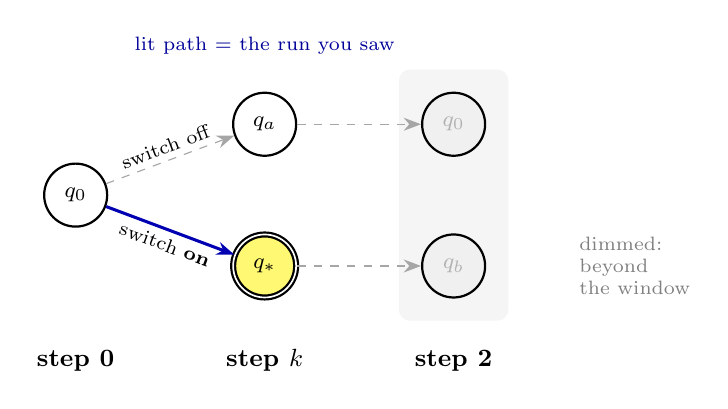
\begin{tikzpicture}[node distance=16mm and 20mm]
  % columns step 0,1,2 ; k = 1
  \node[st] (a0) at (0,0) {$q_0$};
  \node[st] (a1) at (2.4,0.9) {$q_a$};
  \node[goal] (g1) at (2.4,-0.9) {$q_\ast$};
  \node[dead] (a2) at (4.8,0.9) {$q_0$};
  \node[dead] (b2) at (4.8,-0.9) {$q_b$};
  % lit path: a0 -> g1 (goal)
  \draw[lit] (a0) -- node[swlabb]{switch \textbf{on}} (g1);
  % alternate (prevent) path a0 -> a1
  \draw[alt] (a0) -- node[swlab]{switch off} (a1);
  % beyond window edges (dimmed)
  \draw[alt] (g1) -- (b2);
  \draw[alt] (a1) -- (a2);
  % column labels
  \node[col] at (0,-2.1) {step 0};
  \node[col] at (2.4,-2.1) {step $k$};
  \node[col] at (4.8,-2.1) {step 2};
  % dim region after k
  \begin{scope}[on background layer]
    \node[fill=gray!8, rounded corners, fit=(a2)(b2), inner sep=8pt] {};
  \end{scope}
  % goal annotation
  \node[font=\scriptsize, align=center, text=blue!60!black] at (2.4,1.9)
       {lit path = the run you saw};
  \node[font=\scriptsize, align=left] at (7.1,-0.9)
       {\textcolor{gray}{dimmed:}\\ \textcolor{gray}{beyond}\\ \textcolor{gray}{the window}};
\end{tikzpicture}
\caption{Anatomy of a \TRACE{} board. Nodes are machine states; columns are
timesteps; each edge is a switch setting. The thick blue \emph{lit path} is the
observed run, ending on the doubled \emph{goal} node $q_\ast$ that flashes the
target light at step $k$. Dashed edges are untaken (counterfactual) routes; the
shaded region past $k$ is outside the causal window. \emph{Prevent} reroutes the
lit path off $q_\ast$ with the fewest switch changes; \emph{Pin} fixes the switches
that keep every route on a goal node.}
\label{fig:anatomy}
\end{figure}

\subsection{Three readings, three modes}
\label{sec:modes}

The causal question---which earlier switch settings mattered for that flash---has
the three precise readings of Section~\ref{sec:two-questions}. \TRACE{} exposes
each as a one-player mode; the player-facing verbs are deliberately plain. The
\emph{core} mode is \emph{Credit}, the actual-cause object we conjecture aligns
with TempoBench (Conjecture~\ref{conj:corp}); \emph{Prevent} and \emph{Pin} are its
necessity and sufficiency halves, useful both as diagnostics and as the most
immediately playable entry points.

\paragraph{Credit it (actual causation; the core).} \emph{Mark every switch that
actually decided the flash.} A switch is a decider if there is \emph{some} setting
of the other switches---you may move them off their observed values---under which
toggling it flips the flash while, with the switch in place, the flash still fires.
You demonstrate this with a \emph{pair} of runs under that setting (switch in place
vs.\ toggled), the two arms of the contingency. A submission is either one minimal
\emph{actual cause} (Definition~\ref{def:actual}; the witness task) or the cell set
$\Gamma^{\mathrm{ac}}$ (the per-cell union task), graded as in
Section~\ref{sec:scoring}. This is the multi-switch object we \emph{hypothesize}
matches TempoBench's per-cell answers (Conjecture~\ref{conj:corp}) and that escapes
the collapse of Proposition~\ref{prop:pivotal}.

\paragraph{Prevent it (count-only necessity; a strict diagnostic).} \emph{Find a
single switch whose flip---by itself, everything else left as it was---stops the
flash.} That pivotal switch is the cause; a submission is a singleton $\Gamma$,
correct iff it is \emph{valid} (Definition~\ref{def:valid}) and subset-minimal. By
Proposition~\ref{prop:pivotal}, on input-deterministic, input-total controllers
((F2)--(F3))
this is always either a single pivotal switch or the verdict \emph{no pivotal
cell}---no single switch alone stops the flash. The verb matches the predicate:
\emph{Prevent} asks for a switch pivotal \emph{on its own}, \emph{not} for the
smallest group of changes that would prevent the flash. Those differ---in
Puzzle~3 two changes prevent the flash yet no single switch is pivotal, so the
count-only answer is correctly ``no pivotal cell''---which is exactly why bare
necessity is too weak for TCE and why \emph{Credit} is the core.

\paragraph{Pin it (sufficiency; the determining-set object).} The dual:
\emph{lock the fewest switches at their settings so the target light flashes no
matter how the other switches are set.} The locked set is what forces the flash; a
submission is correct iff it is \emph{sufficient} (Definition~\ref{def:determining})
and subset-minimal. \emph{Pin} routinely yields multi-switch answers, and an
actual cause is exactly a switch counterfactually necessary \emph{within} some
such determining set (Section~\ref{sec:two-questions}).

All three are one-player: you only set or mark switches, and the ``for some
setting of the others'' (\emph{Credit}) and ``no matter how the others are set''
(\emph{Pin}) are the grader's quantifiers---finite checks over the same frozen
device---not a live opponent. A live adversary would change the question from
``what caused \emph{this} run'' to ``what can the controller \emph{guarantee}
against \emph{every} environment''---a strategy-level object that needs the
synthesis game rather than the device, kept as a separate variant in
Appendix~\ref{app:flex}, not the core.

\begin{center}
\fbox{\begin{minipage}{0.92\linewidth}
\textbf{Benchmark configurations (to prototype and compare).}\\[2pt]
\textbf{\TRACE-Credit} (core): the actual-cause object---multi-switch answers
conjectured to match TempoBench's per-cell labels (Conjecture~\ref{conj:corp}).\\[2pt]
\textbf{\TRACE-Prevent} (diagnostic): count-only necessity only---single pivotal
switches or the no-pivotal-cell verdict (Proposition~\ref{prop:pivotal}); the
cheapest, strictest mode.\\[2pt]
\textbf{\TRACE-Pin} (diagnostic / dual): determining-set sufficiency only---the
multi-switch ``what forces the flash'' question.
\end{minipage}}
\end{center}

\subsection{The try button: probe and rewind}
\label{sec:probe}

Players act by experiment, not by reading the wiring. \emph{Set} any switches in
the window---to their observed values or to new ones---and press \emph{run}; the
device replays from the start, the light panel recomputes (deterministically, by
(F2)), and you see whether the target flashes and how many switches you changed
from the observed run. One press evaluates the active mode's inner question on
\emph{one} scenario:
\begin{itemize}[nosep]
  \item \emph{Prevent}: did flipping this one switch (others left as observed) stop
        the flash?
  \item \emph{Credit}: under this chosen setting of the other switches, does the
        candidate decide the flash? (A contingency test is a \emph{pair} of
        presses---candidate in place vs.\ toggled.)
  \item \emph{Pin}: with these switches locked and the rest set this way, does the
        flash survive?
\end{itemize}
A single press cannot settle \emph{Pin}'s ``for all other settings'' or
\emph{Credit}'s ``for some setting'' by itself---those quantifiers are the
\emph{grader}'s, discharged by the finite check of
Section~\ref{sec:groundtruth}; a press gives the player evidence about one
scenario, from which they must generalize.

Presses are budgeted, and the budget is what forces \emph{reasoning} over search.
The space of settings over a window of depth $k$ is $2^{\Theta(|I|\,k)}$, so a
budget of only $O(k)$ presses cannot enumerate it: the player must form and test
\emph{compositional} hypotheses about how the device responds, which is the
ability the benchmark means to measure. At $\beta_{\max}=0$ the player must
simulate the device in their head (pure deduction); a very large budget degrades
the game to trial and error. Budget is therefore a difficulty knob
(Section~\ref{sec:difficulty}). One deliberate deviation in the shipped
white-box \emph{human} build must be declared here: since the device is shipped
anyway, the live board simulates freely ($\beta=\infty$; attempts are the
scored resource)---the human analog of the code-equipped agent regime of
Section~\ref{sec:agent}, and like it a \emph{declared condition}, reported
separately. The budgeted construct described above is retained as its own arm
of the human study (and is the regime of the black-box track and of agent
evaluations), so live-board, budgeted, and $\beta=0$ results are never pooled. A submission is read straight off the
panel---marked cells (\emph{Credit}), changed switch (\emph{Prevent}), or locked
switches (\emph{Pin})---so it is gradable identically for people and agents, with
no free text.

\subsection{Winning and scoring}
\label{sec:scoring}

A submission is graded by the formal checker of Section~\ref{sec:groundtruth},
against the \emph{predicate} for the active mode, in one of three granularities.

\begin{description}[leftmargin=3.0cm,style=nextline]
  \item[Native (per mode).] Graded against the active mode's predicate---an
        \emph{actual cause} in \emph{Credit} (Definition~\ref{def:actual}), a
        \emph{valid} cause in \emph{Prevent} (Definition~\ref{def:valid}), a
        \emph{sufficient} set in \emph{Pin} (Definition~\ref{def:determining})---in
        one of three task variants, each with its own predicate:
        \begin{itemize}[nosep,leftmargin=1.4em]
          \item \emph{Witness:} submit one set; full credit iff it is correct
                \emph{and subset-minimal}. Minimality is essential---a non-minimal
                superset scores $0$, so ``spam every cell'' fails.
          \item \emph{All-causes:} submit a family; full credit iff it is exactly
                the set of \emph{all} minimal causes for the mode.
          \item \emph{Per-cell union:} submit the cell set $\Gamma^{\mathrm{ac}}$,
                the union of all minimal causes, graded per cell. This is the
                granularity TempoBench reports; note the union need not itself be a
                single minimal cause, nor decompose into singleton causes.
        \end{itemize}
        The checker accepts \emph{any} correct witness, not a fixed string. Witness
        or per-cell union is the recommended primary metric, depending on whether
        the corpus targets a single explanation or TempoBench-style per-cell scoring.
  \item[Timestep-level (TS).] Against a shipped canonical set, a step scores only
        if its whole predicted switch set matches at that step. This mirrors
        TempoBench's $F_1$(TS) metric---the metric behind its headline TCE
        numbers~\cite{holzer2025tempobench}---and is useful for leaderboards.
  \item[AP-level.] Precision/recall/$F_1$ per switch cell against the canonical
        actual-cause set, mirroring TempoBench's $F_1$(AP)
        metric~\cite{holzer2025tempobench}. A smooth signal for training, but,
        being per-cell, it can give partial credit to an answer that is not a
        correct minimal cause for the mode.
\end{description}

\paragraph{Why set-valued grading matters.} Answers are genuinely non-unique:
\emph{Credit} and \emph{Prevent} can have several incomparable causes (Puzzle~4),
and \emph{Pin} several determining sets (Puzzle~3). Grading the witness task
against one stored string would mark a correct minimal answer wrong for merely
differing from it; native grading checks the \emph{predicate} instead---a facility
ARC-style exact-match grading lacks, and one the formal backbone provides.
TempoBench's $F_1$(AP) sidesteps this for the per-cell union task, but being
per-cell it gives partial credit to non-minimal or partly-wrong answers;
\TRACE{}'s native predicate grading is what we add. A canonical set
(e.g.\ the lexicographically least) is still shipped for the TS and AP
granularities, but the primary score is native.

\paragraph{Attempts.} As in ARC-AGI, a puzzle allows a few submissions and is
\emph{solved} if any attempt earns full native credit, bounding lucky guessing
while tolerating one slip.

\subsection{Difficulty knobs}
\label{sec:difficulty}

\TRACE{} difficulty is set by observable, reportable features, so a corpus can be
stratified and calibrated against human panels exactly as ARC-AGI-2 is.

\begin{center}
\small
\begin{tabular}{@{}lll@{}}
\toprule
\textbf{Knob} & \textbf{Effect on difficulty} & \textbf{Source} \\
\midrule
effect depth $k$ & longer causal window, more credit assignment & TempoBench \\
\# automaton states & richer internal dynamics to simulate & TempoBench \\
transition count & denser branching & TempoBench \\
causal-input count $|\Gamma^\star|$ & larger true cause & TempoBench \\
trace diversity (\# distinct inputs) & more candidate cells & TempoBench \\
trace length $n$ & more distractor context & \TRACE{} \\
probe budget $\beta_{\max}$ & less brute-force checking & \TRACE{} \\
mode (\emph{Credit}/\emph{Prevent}/\emph{Pin}) & actual cause / necessity / sufficiency & \TRACE{} \\
closeness order & count-only vs.\ profile (App.~\ref{app:flex}) & framework \\
\bottomrule
\end{tabular}
\end{center}

As in ARC-AGI-2, the generator should discard instances solvable without
reasoning---e.g.\ those whose target is unconditional ($\Gamma^\star=\emptyset$),
or whose cause is a single literal in the same column as the effect---and
calibrate the retained set so that humans reliably solve it while the cheapest
brute-force probe strategy does not.

\subsection{Five worked puzzles}
\label{sec:worked}

We trace the evaluation of five example puzzles. Each device is described in plain
terms (its formal transition function stays under the hood) and drawn as a trellis
in the style of Figure~\ref{fig:anatomy}: the blue lit path is the observed run,
the doubled yellow $q_\ast$ is the target flash, and dashed edges are untaken
routes. Closeness counts changed input cells, and for each puzzle we report all
three readings---\emph{Credit} (actual cause, the core), \emph{Prevent} (count-only
necessity), and \emph{Pin} (sufficiency). All five devices are encoded as HOA
transducer artifacts in the repository's verification suite, and every answer
reported below---including the modified-variant verdicts discussed in
Section~\ref{sec:two-questions}---is reproduced mechanically by the reference
checker from those artifacts (exhaustive enumeration over the window cells), not
by hand simulation. Puzzles~1--2 have the three
readings agree; Puzzles~3--5 show them diverge---the reason the core is actual
causation, not bare necessity---with Puzzle~5 a genuinely multi-step ($k{=}2$)
case.

\paragraph{Puzzle 1 (one pivotal switch; tutorial).}
\emph{Device:} a button and a lamp; the lamp flashes one step after the button is
pressed. Window $\{0,1\}$, target $=$ lamp at step $1$.
\begin{center}
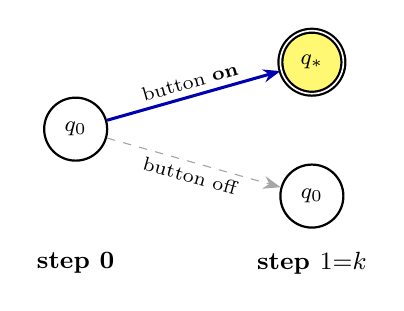
\begin{tikzpicture}
  \node[st] (s0) at (0,0) {$q_0$};
  \node[goal] (f1) at (3,0.85) {$q_\ast$};
  \node[st] (r1) at (3,-0.85) {$q_0$};
  \draw[lit] (s0) -- node[swlab]{button \textbf{on}} (f1);
  \draw[alt] (s0) -- node[swlabb]{button off} (r1);
  \node[col] at (0,-1.7) {step 0};
  \node[col] at (3,-1.7) {step $1{=}k$};
\end{tikzpicture}\\[1pt]
{\footnotesize Lit blue path $=$ observed run; doubled yellow $q_\ast$ $=$ the target
flash; dashed $=$ the \emph{Prevent} reroute. One change (button off) leaves the goal.}
\end{center}
\emph{Credit:} with everything else fixed, toggling the button at step $0$ flips
the flash, so $\{(0,\text{button})\}$ is the lone actual cause. \emph{Prevent:}
releasing the button at step $0$ (one change) stops the flash; pressing at step $1$
does nothing---same pivotal switch. \emph{Pin:} locking the button on at step $0$
forces the flash regardless of step $1$; same singleton. All three readings agree.

\paragraph{Puzzle 2 (delayed cause with a distractor).}
\emph{Device:} two switches $a,b$ and a lamp \emph{done}; the lamp flashes exactly
two steps after $a$ is set, and $b$ does nothing. Window $\{0,1,2\}$, target $=$
\emph{done} at step $2$.
\begin{center}
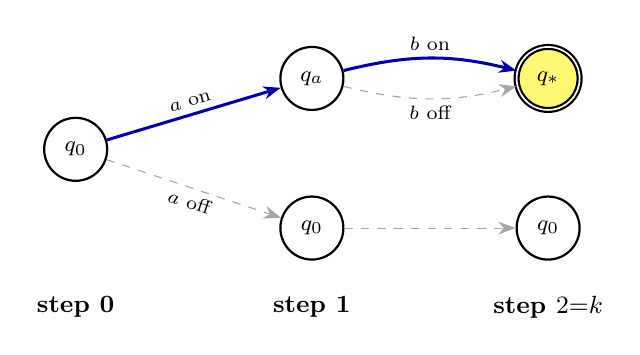
\begin{tikzpicture}
  \node[st] (s0) at (0,0) {$q_0$};
  \node[st] (sa) at (3,0.9) {$q_a$};
  \node[st] (s01) at (3,-1.0) {$q_0$};
  \node[goal] (g) at (6,0.9) {$q_\ast$};
  \node[st] (s02) at (6,-1.0) {$q_0$};
  \draw[lit] (s0) -- node[swlab]{$a$ on} (sa);
  \draw[alt] (s0) -- node[swlabb]{$a$ off} (s01);
  \draw[lit] (sa) to[bend left=14] node[swlab]{$b$ on} (g);
  \draw[alt] (sa) to[bend right=14] node[swlabb]{$b$ off} (g);
  \draw[alt] (s01) -- (s02);
  \node[col] at (0,-2.0) {step 0};
  \node[col] at (3,-2.0) {step 1};
  \node[col] at (6,-2.0) {step $2{=}k$};
\end{tikzpicture}\\[1pt]
{\footnotesize $a$ at step 0 is pivotal (the $a$-off route never reaches $q_\ast$);
$b$ is a distractor---\emph{both} $b$ edges from $q_a$ land on the flash.}
\end{center}
\emph{Credit/Prevent/Pin:} only $a$ at step $0$ matters---toggling it (under any
setting of $b$) flips the flash, it alone prevents, and it alone forces---so all
three readings give $\{(0,a)\}$. This is genuine delayed credit assignment
($k{=}2$) on which the readings still coincide; the traps are the two-step
\emph{delay} and the present-but-irrelevant $b$, which bait a recency or same-step
guess.

\paragraph{Puzzle 3 (overdetermination: the modes diverge).}
\emph{Device:} switches $a,b$ and a lamp \emph{fire}; the lamp flashes one step
after \emph{either} switch is set. Both are set at step $0$. Window $\{0,1\}$,
target $=$ \emph{fire} at step $1$.
\begin{center}
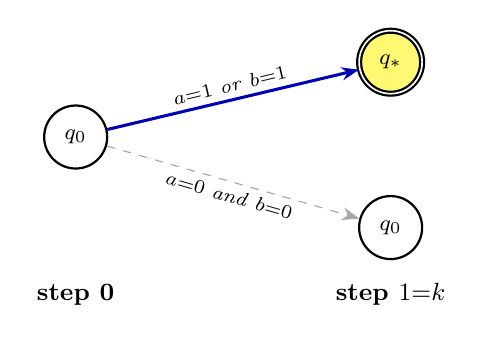
\begin{tikzpicture}
  \node[st] (s0) at (0,0) {$q_0$};
  \node[goal] (g) at (4,0.95) {$q_\ast$};
  \node[st] (n) at (4,-1.15) {$q_0$};
  \draw[lit] (s0) -- node[swlab]{$a{=}1$ \emph{or} $b{=}1$} (g);
  \draw[alt] (s0) -- node[swlabb]{$a{=}0$ \emph{and} $b{=}0$} (n);
  \node[col] at (0,-2.0) {step 0};
  \node[col] at (4,-2.0) {step $1{=}k$};
\end{tikzpicture}\\[1pt]
{\footnotesize Only setting \emph{both} switches off (two changes) escapes the
flash, so no single change prevents it---\emph{no pivotal cell} for
\emph{Prevent}. \emph{Credit}: each switch is pivotal once the other is held
off, so each is an actual cause. \emph{Pin}: $a{=}1$ alone, or $b{=}1$ alone,
already forces it (two determining sets).}
\end{center}
\emph{Prevent:} clearing $a$ leaves $b$, which still fires; clearing $b$ is
symmetric; only the two-change removal escapes, while every one-change removal
preserves the flash. So no single switch is pivotal and $\Causes^{\le n}=\emptyset$:
count-only necessity reports \emph{no pivotal cell}, and since actual causes
exist (next), the effect is genuinely overdetermined. \emph{Credit:} hold $b$ off (a
contingency) and $a$ becomes pivotal; hold $a$ off and $b$ becomes pivotal; so
\emph{both} $\{(0,a)\}$ and $\{(0,b)\}$ are actual causes---the multi-cell
shape a Halpern--Pearl key can report, recovered exactly where \emph{Prevent}
saw nothing.
\emph{Pin:} locking $a$ on forces the flash no matter what $b$ does (and
symmetrically), so there are \emph{two} determining sets $\{(0,a)\}$ and
$\{(0,b)\}$. The one instance reads as ``no single switch was necessary''
(\emph{Prevent}), ``each switch is a cause'' (\emph{Credit}), and ``either
alone suffices'' (\emph{Pin})---the collapse of bare necessity, and why the
core is actual causation.

\paragraph{Puzzle 4 (a guard: the modes diverge the other way).}
\emph{Device:} a request switch $req$, a cancel switch $cancel$, and a lamp
\emph{grant}; the lamp flashes at a step exactly when $req$ is set \emph{and}
$cancel$ is not, at that same step. At step $0$, $req$ is set and $cancel$ is not.
Window $\{0\}$, target $=$ \emph{grant} at step $0$.
\begin{center}
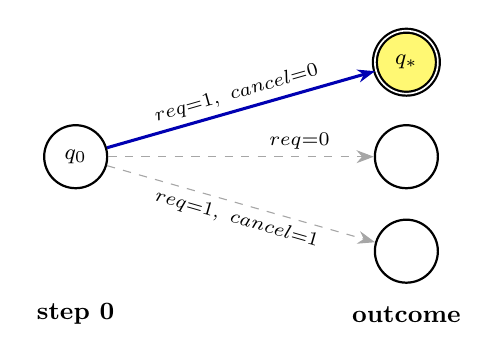
\begin{tikzpicture}
  \node[st] (s0) at (0,0) {$q_0$};
  \node[goal] (g) at (4.2,1.2) {$q_\ast$};
  \node[st] (n1) at (4.2,0) {};
  \node[st] (n2) at (4.2,-1.2) {};
  \draw[lit] (s0) -- node[swlab]{$req{=}1,\ cancel{=}0$} (g);
  \draw[alt] (s0) -- node[swlab,pos=0.72]{$req{=}0$} (n1);
  \draw[alt] (s0) -- node[swlabb]{$req{=}1,\ cancel{=}1$} (n2);
  \node[col] at (0,-2.0) {step 0};
  \node[col] at (4.2,-2.0) {outcome};
\end{tikzpicture}\\[1pt]
{\footnotesize Only $req{=}1,cancel{=}0$ flashes \emph{grant} ($q_\ast$). Flipping
\emph{either} switch escapes---two pivotal switches (\emph{Prevent}); \emph{Pin}
must lock \emph{both} to stay on $q_\ast$.}
\end{center}
\emph{Prevent:} clearing $req$ stops the flash, and so does setting $cancel$; each
single change works, so there are \emph{two} pivotal switches $\{(0,req)\}$ and
$\{(0,\neg cancel)\}$. \emph{Credit:} each is pivotal under the actual setting of
the other, so both are actual causes---necessity and actual cause here return the
guard's parts \emph{separately}. \emph{Pin:} neither alone suffices (with $req$
locked on, a set $cancel$ still kills the flash), but locking \emph{both} forces
it, so the single determining set is the pair $\{(0,req),(0,\neg cancel)\}$---
sufficiency returns the parts \emph{together}. This is why a string-match grader is
wrong in every mode, and why a corpus must declare which question it asks
(Section~\ref{sec:scoring}, Appendix~\ref{app:flex}). \emph{A caveat:} with $k{=}0$
the cause sits in the same column as the effect, so an evaluation corpus would
\emph{discard} this instance under the trivial-instance filter of
Section~\ref{sec:difficulty}; we keep it here only because it isolates the
necessity/sufficiency divergence in the smallest possible device. Puzzle~5 shows
the same divergence at genuine temporal depth.

\paragraph{Puzzle 5 (delayed overdetermination; a genuinely multi-step divergence).}
\emph{Device:} switch $a$ (read at step $0$) and switch $b$ (read at step $1$) and
a lamp \emph{fire}; \emph{fire} flashes at step $2$ if $a$ was set at step $0$
\emph{or} $b$ at step $1$. Observed: $a$ set at $0$, $b$ set at $1$, \emph{fire} at
$2$. Window $\{0,1,2\}$, target $=$ \emph{fire} at step $2$.
\begin{center}
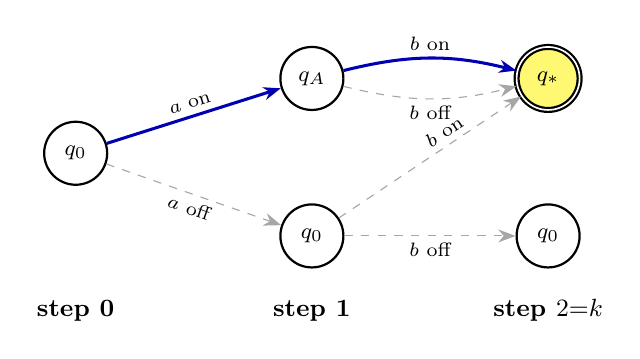
\begin{tikzpicture}
  \node[st] (s0) at (0,0) {$q_0$};
  \node[st] (sa) at (3,0.95) {$q_A$};
  \node[st] (s0b) at (3,-1.05) {$q_0$};
  \node[goal] (g) at (6,0.95) {$q_\ast$};
  \node[st] (nf) at (6,-1.05) {$q_0$};
  \draw[lit] (s0) -- node[swlab]{$a$ on} (sa);
  \draw[alt] (s0) -- node[swlabb]{$a$ off} (s0b);
  \draw[lit] (sa) to[bend left=14] node[swlab]{$b$ on} (g);
  \draw[alt] (sa) to[bend right=14] node[swlabb]{$b$ off} (g);
  \draw[alt] (s0b) -- node[swlab,pos=0.62]{$b$ on} (g);
  \draw[alt] (s0b) -- node[swlabb]{$b$ off} (nf);
  \node[col] at (0,-2.0) {step 0};
  \node[col] at (3,-2.0) {step 1};
  \node[col] at (6,-2.0) {step $2{=}k$};
\end{tikzpicture}\\[1pt]
{\footnotesize From $q_A$ ($a$ already on) \emph{both} $b$-edges reach the flash;
from the $a$-off $q_0$, only $b$ on reaches it. Each cause sits at a
\emph{different} timestep.}
\end{center}
\emph{Prevent:} clearing $a$ at step $0$ alone still fires ($b$ at $1$ remains), and
clearing $b$ at step $1$ alone still fires ($a$ at $0$ remains); no single change
prevents, so $\Causes^{\le n}=\emptyset$---\emph{no pivotal cell}, with the
effect again genuinely overdetermined, exactly as in
Puzzle~3 but now across two timesteps. \emph{Credit:} hold $b$ at $1$ off and $a$ at
$0$ becomes pivotal; hold $a$ at $0$ off and $b$ at $1$ becomes pivotal; so both
$\{(0,a)\}$ and $\{(1,b)\}$ are actual causes---a multi-cell answer spread
\emph{across time}, recovered where \emph{Prevent} saw nothing. \emph{Pin:} $a$ at
$0$ alone forces the flash, and $b$ at $1$ alone forces it, giving two determining
sets $\{(0,a)\}$ and $\{(1,b)\}$. This is the case the benchmark is built
for---credit assignment across a delay, where count-only necessity collapses and
the actual-cause core does not.

\section{Playing as an AI Agent}
\label{sec:agent}

The same puzzle is exposed to an AI agent through a text protocol that mirrors the
human device one-to-one. Parity is the point: within each \emph{declared
condition}---a track (white- or black-box), a mode, and one declared
Halpern--Pearl variant---the human and the agent receive \emph{the same
information} and the same probe tool, take the same actions, and are graded by
the same checker on the same answer format. Results are never compared across
undeclared conditions: a human score under one variant is matched only against
an agent score under the same variant, and the live-board human regime is
matched against the corresponding free-simulation agent regime
(Section~\ref{sec:probe}). Nothing in the agent interface
reveals the answer key or $\varphi$.

\subsection{Observation: two tracks}

\paragraph{White-box (primary).} The primary track ships the device
explicitly to \emph{both} players---the agent gets the transition table or the
raw HOA text TempoBench uses, the human sees the trellis of
Figure~\ref{fig:anatomy}. This is the information setting of TempoBench's TCE,
and it isolates simulation-plus-counterfactual reasoning with no
identification burden. One caveat governs its interpretation: an agent
permitted to execute code can mechanize the grader's reachability search, so
white-box agent evaluations must declare the tool regime---tool-less runs
measure reasoning, code-equipped runs serve as a solver ceiling.

\paragraph{Black-box (discovery track).} The second track withholds the
machine from human and agent alike; both see only the switch and light panels
of the observed run, the target, the mode, and the budgets, and learn how the
device behaves only through the probe tool below. This defeats checker
mechanization and adds system identification to the task---deliberately, but
it changes what a score means: an error may reflect underdetermination rather
than bad reasoning if two devices consistent with everything observed disagree
on the answer. The track therefore carries an \emph{identifiability
requirement}: an instance is admitted only if every device consistent with the
observed run and with the information obtainable within the probe budget
yields the same native answer. Enforcing this in the generator is roadmap
step~V5; black-box scores are reported as measuring
identification-plus-reasoning jointly.

The agent's observation (machine field present in white-box, absent in
black-box):
\begin{quote}\small\ttfamily
\{\\
\ \ "switches": ["a","b"], "lights": ["fire"],\\
\ \ "run": [ \{"t":0,"a":1,"b":1,"fire":0\}, \{"t":1,"a":0,"b":0,"fire":1\} ],\\
\ \ "target": \{ "light":"fire", "step":1 \},\\
\ \ "mode": "credit", "window": [0,1], "probe\_budget": 8, "max\_attempts": 2\\
\}
\end{quote}
The \texttt{mode} field selects \emph{credit}, \emph{prevent}, or \emph{pin};
the agent is told the rules, the scoring granularity, and the budgets.

\paragraph{A modality caveat.} The human reads a moving board; the agent reads
JSON. This is a difference in \emph{presentation}, not in information, but
spatial-versus-textual encoding could itself shift the measured human--agent gap, so
a careful study should control for it---e.g.\ by also giving humans the JSON and
agents a rendered board.

\subsection{Action and answer}

The agent answers with a grouped, by-step constraint set $\Gamma$, where each cell
is a (timestep, variable\,:\,value) entry---so a negative-literal cause such as
$(0,\neg cancel)$ is simply \texttt{"cancel":0}, and Puzzle~4's guard encodes
cleanly:
\begin{quote}\small\ttfamily
\emph{credit}:\ \ \{ "cause": \{ "0": \{"req":1,"cancel":0\} \} \}\\
\emph{prevent}: \{ "pivot": \{ "0": \{"req":1\} \}, "no\_pivot": false \}\\
\emph{pin}:\ \ \ \ \ \{ "lock": \{ "0": \{"req":1,"cancel":0\} \} \}
\end{quote}
In \emph{credit} the entries are one minimal actual cause or the union
$\Gamma^{\mathrm{ac}}$; in \emph{pin}, the switches to lock. In \emph{prevent},
\texttt{pivot} names the pivotal cell \emph{at its actual value}---the cell
whose flip (to its negation; inputs are binary) stops the flash---and the
boolean \texttt{no\_pivot} lets the agent give Puzzle~3's correct
no-pivotal-cell verdict instead. In every mode the cells are stated at actual
values; the grader supplies the flips. Grouping by step makes AP- and TS-level
scoring direct.

\subsection{The probe tool}

To match the human ``run'' button, the agent may call a \emph{probe} tool:
\begin{quote}\small\ttfamily
probe(\{ "0": \{"a":0\} \})\ \ $\to$\ \ \{ "lights": [...recomputed...], "target\_flashes": false, "switches\_changed": 1 \}
\end{quote}
The tool is the programmatic equivalent of the human run button of
Section~\ref{sec:probe}, budgeted identically: it sets the named switch cells,
re-simulates deterministically, and returns the recomputed lights, the target
status, and the change count. A \emph{credit} contingency test is a \emph{pair}
of probes under one setting of the other cells---candidate in place vs.\
toggled---costing two against the budget and exhibiting both arms (AC2(a),
AC2(b)) of Definition~\ref{def:actual}. Two evaluation regimes follow:
\begin{itemize}[nosep]
  \item \textbf{Tool-use regime} ($\beta_{\max}>0$): the agent probes to
        discover how the device responds and then reasons---guided
        experimentation, the temporal analog of running code to test a
        hypothesis. In the black-box track this is the \emph{only} way to learn
        the machine, so $\beta_{\max}>0$ is required there.
  \item \textbf{Pure-reasoning regime} ($\beta_{\max}=0$): with the machine
        shown (white-box track), the agent must \emph{simulate} it over the
        window and reason about the causal question with no execution. This
        isolates internal world-modeling and is the harder, more ARC-like
        setting. ($\beta_{\max}=0$ with the machine hidden is excluded: one
        run does not fix the counterfactuals.)
\end{itemize}

\subsection{Verifiable reward}

Because grading is the formal checker, the reward is computed without a human or a
reference model: full reward iff the submission is correct for the active mode
(native), or graded partial credit (AP/TS modes). This makes \TRACE{} a
\emph{verifiable-reward} environment suitable both for evaluation and for
reinforcement learning, with no reward-model drift. The per-call cost is the
mode-dependent cost of Section~\ref{sec:groundtruth}---polynomial in the explicit
automaton and $k$ for sufficiency and necessity, exponential in $|I|\cdot k$ for
the core \emph{Credit} mode (the contingency search)---and the minimality test adds
$2^{|\Gamma|}$ calls, small because minimal causes are small. The benchmark
targets small-window instances on which this is designed to be tractable at
training scale, with \emph{Credit} the costliest mode; the measured envelope of
the reference implementation (sub-second median full-key computation through
$(|I|,k)=(2,3)$, $1$--$10$\,s at $(2,4)$ and $(3,2)$) bounds the regime the
verifiable-reward claim currently extends to.

\subsection{Why the task is hard for current models---and where it is not}

The task is designed to resist the failure modes that inflate scores on text
benchmarks. No natural-language world knowledge applies: each device is freshly
generated, so there is no fact to retrieve---though instances are drawn from a
fixed SYNTCOMP-derived distribution whose controller families (arbiters,
AMBA-style protocols) have structure a model could in principle learn, a
distributional prior the evaluation should measure rather than assume away.
Solving a puzzle requires (i) \emph{learning or simulating}
a finite-state machine over a window---multi-step state tracking that language
models do unreliably as depth grows, and which in the black-box track must first be
recovered from probes---and (ii) \emph{counterfactual} reasoning that is provably
non-monotone (Remark~\ref{rem:nonmonotone}). We are careful about what
non-monotonicity buys: it shows that no \emph{exact} greedy or single-pass
heuristic can be correct in general (Puzzles~2, 3, and~5), but it does \emph{not}
by itself show that \emph{approximate} shortcuts score low, so we treat
``memorization-proof'' as a design goal to confirm empirically, not a theorem.

The closest existing evidence is TempoBench's own TCE results: aggregated
across the evaluated models, timestep-level $F_1$ is $65.6\%$ on TCE-normal but
only $7.5\%$ on TCE-hard~\cite{holzer2025tempobench}---models clearly
``understand the task'' yet degrade sharply as the device grows. So the
ARC-like profile (near-floor machine scores against high human solve rates)
holds at the \emph{hard} stratum, not uniformly; on easy instances the models
evaluated in the October 2025 TempoBench paper already do well. Two caveats
temper even that: those are $F_1$ scores at the timestep granularity
(TempoBench also reports a per-cell AP-level $F_1$, which is more permissive),
and both give partial credit across the trace relative to \TRACE{}'s
exact-answer native predicate; and the numbers predate any \TRACE{}-specific
calibration. We therefore position \TRACE{} as targeting the hard stratum by
construction (large $k$, more states, tight or zero probe budget) and leave
the human--agent gap to roadmap steps~V6--V7.

\section{The ARC-AGI Analogy, Made Precise}
\label{sec:arc}

\TRACE{} is deliberately built to the ARC-AGI template, and the comparison
clarifies both what it borrows and what the formal backbone adds.

\paragraph{What it shares with ARC-AGI.} Small, self-contained instances that fit
on a screen; a novel ``rule of the world'' per puzzle so success cannot come from
recall; a fixed, simple answer format scored automatically; a few-attempt
protocol; difficulty calibrated against human panels; and the target property of
being \emph{approachable for people yet hard for machines}---a design goal to
be validated by the human pilot (roadmap step~V6), not assumed---testing fluid
reasoning rather than crystallized knowledge~\cite{chollet2019measure}.

\paragraph{What the formal backbone adds.} Three properties follow from grading
against a predicate rather than a stored grid:
\begin{enumerate}[label=(\arabic*),nosep]
  \item \textbf{Decidable, generated ground truth.} ARC tasks are hand-authored
        and their answers hand-drawn. \TRACE{} answers are \emph{computed and
        checked} against the actual-cause predicate (Section~\ref{sec:groundtruth})
        from synthesized artifacts---certified against that predicate, and
        conjectured to equal CORP's labels (Conjecture~\ref{conj:corp})---so a
        corpus can be \emph{procedurally generated at scale} with labels correct by
        construction of the checker and with dialed-in difficulty.
  \item \textbf{Set-valued correctness.} ARC accepts one output grid.
        Temporal answers can be genuinely non-unique---several actual causes in
        \emph{Credit} (Puzzles~3--5), pivotal switches in \emph{Prevent}
        (Puzzle~4), or determining sets in \emph{Pin} (Puzzle~3)---and the native
        grader accepts \emph{any} correct minimal witness, a more faithful notion
        of ``correct reasoning'' than exact match, available only because the
        predicate is decidable.
  \item \textbf{A built-in experiment affordance.} The probe sandbox gives a
        principled, budgetable notion of ``testing a hypothesis'' that ARC's
        static grids do not, and that cleanly separates pure reasoning
        ($\beta_{\max}=0$) from guided experimentation.
\end{enumerate}

\paragraph{What is different in kind.} The analogy is to \emph{format and rigor},
not to the cognitive loop. ARC tests \emph{inductive} spatial abstraction over
\emph{Core Knowledge} priors (objectness, geometry,
counting)~\cite{chollet2019measure}: infer a static rule from examples. \TRACE{} tests \emph{deductive/abductive} temporal credit
assignment---simulate or probe a hidden machine over time and reason
counterfactually about which inputs decided an event. These are complementary axes
of fluid intelligence; an agent strong on one need not be strong on the other, and
we borrow ARC's packaging without claiming it measures the same thing.

\begin{center}
\small
\begin{tabular}{@{}lll@{}}
\toprule
 & \textbf{ARC-AGI} & \textbf{\TRACE{}} \\
\midrule
Instance & input/output grid pairs & reactive device + switch/light run + target flash \\
Reasoning axis & spatial abstraction & temporal actual causation (necessity + sufficiency) \\
Answer & an output grid & a set of timestep-indexed switches \\
Ground truth & hand-authored & computed; checked vs.\ predicate ($\approx$ CORP, Conj.~\ref{conj:corp}) \\
Uniqueness & single grid & set-valued (any minimal cause) \\
Generation & human design & procedural from synthesized artifacts \\
Grading & exact-grid match & actual-cause / validity + minimality predicate \\
Experiment & none & budgeted counterfactual probe \\
Priors tested & Core Knowledge & machine simulation + intervention \\
Calibration & timed human panels & timed human panels (same recipe) \\
\bottomrule
\end{tabular}
\end{center}

\section{Roadmap: From Design to Benchmark (TODO)}
\label{sec:roadmap}

The formal design is complete; what follows is the ordered list of validation
and build steps that turn it into a released benchmark. Each step is stated as
a falsifiable TODO with its success criterion; steps V1--V2 are the gatekeepers
for every TempoBench-equivalence claim in this paper.

\begin{enumerate}[label=\textbf{V\arabic*.},leftmargin=2.6em]
  \item \textbf{Artifact audit ((F1)--(F3)).} Parse the released TempoBench HOA
        artifacts and check, per file: that it is an implementation rather than
        a specification monitor (F1), input-determinism (F2), and
        input-totality (F3). Report the fraction of the corpus satisfying each.
        \emph{Success:} a quantified scope for Proposition~\ref{prop:pivotal}
        and Conjecture~\ref{conj:corp}; failures filtered or the claims
        narrowed accordingly. \emph{Status:} the audit is implemented and
        validated against labelled positive and negative controls
        (Remark~\ref{rem:f1f2}); the one publicly available artifact passes
        all three checks; corpus rates await the dataset's re-release.
  \item \textbf{CORP correspondence (Conjecture~\ref{conj:corp}).} Run
        TempoBench's key generation (its Algorithm~1, which invokes
        \texttt{corp}~\cite{holzer2025tempobench,finkbeiner2024corp}) on a
        representative sample of (F1)--(F3) instances and compare its per-cell
        keys with $\Gamma^{\mathrm{ac}}$. Also pin down, from
        \cite{coenen2022temporal}, whether the underlying contingency
        discipline permits non-actual values, as Definition~\ref{def:actual}
        does. \emph{Success:} per-cell agreement rate with disagreements
        published as failure cases; on disagreement, either the definition or
        the alignment claim is revised. \emph{Status:} the definitional
        question is resolved---CORP's contingencies are modified-variant,
        output-valued, and actual-valued (Section~\ref{sec:two-questions})---so
        the conjecture cannot be discharged definitionally; per-cell agreement
        is exact on the single available keyed instance; corpus-scale
        comparison awaits the dataset's re-release, with overdetermined
        instances the predicted divergence class. Whether the shipped keys
        were generated with CORP's contingency toggle enabled has been put to
        the TempoBench authors.
  \item \textbf{Grader implementation and profiling.} Implement the checker of
        Appendix~\ref{app:schema}; measure runtime versus $|I|$ and $k$ for
        each mode; publish the tractable $(|I|,k)$ envelope that the
        verifiable-reward claim of Section~\ref{sec:agent} is then restricted
        to. \emph{Status:} done at reference scale. The grader implements
        every mode from its definition (\emph{Prevent} by closest-removal
        search over Definition~\ref{def:valid} directly---on the worked
        puzzles its accepted singletons coincide exactly with the pivot sets,
        i.e.\ Proposition~\ref{prop:pivotal} is checked against the raw
        definition rather than assumed), reproduces the five worked puzzles
        and the public TempoBench instance end-to-end from HOA artifacts,
        accepts every published witness and rejects every strict superset,
        and is profiled to the envelope reported in
        Section~\ref{sec:groundtruth}. Production-scale optimization within
        that envelope remains.
  \item \textbf{Generator and corpus statistics.} Build the generator
        (P1--P6), produce a prototype corpus, and report: instance counts per
        difficulty stratum; the frequency of the no-pivotal-cell verdict,
        split into overdetermined versus input-unconditional instances; the
        per-cell agreement rate of \emph{Credit} and \emph{Pin}
        (Section~\ref{sec:two-questions})---a per-cell disagreement instance,
        if found, is the example that justifies \emph{Credit} specifically;
        and the trivial-instance discard rate. \emph{Status:} prototyped on
        randomly generated input-deterministic, input-total transducers
        (\emph{not} SYNTCOMP syntheses---corpus realism is deliberately not
        claimed): 139 generated, 107 retained ($23\%$ discarded by the
        trivial-instance filter), every retained instance re-passing the
        (F1)--(F3) audit; no-pivotal-cell verdicts split 11 overdetermined
        versus 4 input-unconditional; \emph{Credit} and \emph{Pin} per-cell
        unions agreed on all 107; original-versus-modified keys diverged on
        $59\%$. The same statistics on real synthesized artifacts await the
        TempoBench corpus.
  \item \textbf{Black-box identifiability enforcement.} Implement the
        admission check of Section~\ref{sec:agent}: an instance enters the
        black-box track only if all devices consistent with the observed run
        and budget-reachable probe information agree on the native answer.
        Report how restrictive the check is in practice. \emph{Status:} the
        admission check is implemented exhaustively within a declared device
        family (sound one-sidedly: inadmissibility under full-budget
        information implies inadmissibility for every smaller budget) and
        behaves correctly on known-identifiable and known-underdetermined
        controls; on random two-state, one-input instances with three probes
        it admitted $0$ of $10$---the check is severely restrictive, and
        black-box corpora will need probe-aware instance selection.
  \item \textbf{Human pilot and calibration.} Following
        ARC-AGI-2~\cite{chollet2025arcagi2}: recruit a panel, present puzzles
        under a time limit and the standard attempt budget, retain an
        evaluation instance only if reliably solved by multiple participants,
        and report per-stratum solve rates against the difficulty knobs and
        the active mode. This is the test of the ``approachable for humans''
        hypothesis, including for \emph{Credit}, whose contingency search may
        be the hardest mode for non-experts.
  \item \textbf{Agent baselines.} Evaluate, in both tracks: prompted models
        with the probe tool; prompted models in the pure-reasoning regime
        ($\beta_{\max}=0$, white-box); reasoning-trained models; and the
        generator's own search as a non-learning ceiling. Report native, TS,
        and AP scores per mode, probe usage, and the no-pivotal-cell
        recognition rate. Primary metric: native solve rate; the human--agent
        gap per stratum is the quantity the benchmark exists to track.
  \item \textbf{Release.} Corpus, checker, canonical keys, and the JSON
        protocol of Appendix~\ref{app:schema}, versioned so that V1--V7
        results are reproducible.
\end{enumerate}

\paragraph{What success would show.} A useful benchmark exhibits a wide
human--agent gap that narrows only with genuine improvements in temporal and
counterfactual reasoning, and resists brute-force probing (hence the budget).
If agents close the gap by probing exhaustively, tighten $\beta_{\max}$; if
they close it by a heuristic, the non-monotonicity result
(Remark~\ref{rem:nonmonotone}) says a heuristic cannot be exactly correct in
general, so discriminating instances can be surfaced.

\section{Limitations}
\label{sec:limitations}

\begin{itemize}[nosep]
  \item \textbf{Conditional alignment.} Every TempoBench-equivalence claim
        rests on (F1)--(F3) and Conjecture~\ref{conj:corp}. The (F1)--(F3)
        audit is implemented, control-validated, and passes on the one publicly
        available artifact; the conjecture's definitional half is resolved
        \emph{negatively} (CORP uses the modified contingency discipline,
        Section~\ref{sec:two-questions}), while its per-cell half holds
        exactly on the single available keyed instance. If the per-cell claim
        fails at corpus scale---expected, if at all, on overdetermined
        instances---the grader still defines a clean, decidable game over
        whatever $A_{\HOA}$ \emph{is}, but the claim of TempoBench equivalence
        lapses (or is restated under the modified discipline) and \TRACE{}
        stands as an independent trellis-causation benchmark.
  \item \textbf{Generation cost.} Computing the actual-cause key compounds a
        minimal-cause search with an outer contingency search; each underlying
        simulation is polynomial in the explicit (expanded) automaton and $k$,
        but the searches are exponential in $|I|\cdot k$ in the worst case
        (Section~\ref{sec:groundtruth}). The difficulty knobs keep production
        tractable but cap instance size.
  \item \textbf{The simplest mode is degenerate by design.} Count-only
        \emph{Prevent} collapses on input-deterministic, input-total
        controllers (Proposition~\ref{prop:pivotal}); we retain it only as a
        strict diagnostic, and the core is actual causation. A reader expecting
        necessity to be the TCE object should note this is exactly why it is
        not.
  \item \textbf{A genuine ceiling: one-player reach.} The frozen device is
        adequate for trace-level point-effect causes, which is the whole of TCE,
        but \emph{cannot} express liveness or strategy-level causes (``was this
        standing controller commitment necessary against every environment'');
        those require the two-player reverse parity game of
        Appendix~\ref{app:flex}, where polynomial-time \emph{generation} is lost.
  \item \textbf{Black-box scores bundle identification with reasoning.} This
        is deliberate---it is what makes the probe budget meaningful---and it
        is why the black-box track carries the identifiability requirement of
        Section~\ref{sec:agent} (enforced by roadmap step~V5) and why
        white-box is the primary reasoning track.
  \item \textbf{Closeness is a declared choice.} Count-only closeness is canonical
        but not forced; profile refinement (Appendix~\ref{app:flex}) can change
        which removals are ``closest'' and hence, at the margin, validity. A corpus
        must declare its order.
  \item \textbf{Playability is a hypothesis until the pilot runs.} What is
        machine-verified about the playable build is mathematics and parity:
        render--simulation equivalence, oracle-equality of every on-screen
        verdict, submission round-trip per declared variant, and
        candidate-space safety. ``Approachable for humans,'' legibility of
        generated boards, and the teaching value of the level ramp are
        \emph{empirical} properties, conditional on the human pilot (roadmap
        step~V6), which has not yet run; until it does, every such phrase in
        this paper should be read as design intent. Generated instances
        additionally pass only a heuristic legibility gate (window-size,
        fan-out, and accepted-witness caps), not human calibration, and the
        prototype corpus statistics come from random transducers, not
        SYNTCOMP syntheses.
\end{itemize}

\section{Conclusion}
\label{sec:conclusion}

We turned a formal, frame-relative notion of temporal cause into a benchmark.
Specializing to point effects under input-only counterfactuals re-grounds the
TempoBench TCE task as a self-contained, finite construction on three decidable
causal objects---necessity, sufficiency, and actual causation---of which actual
causation is the one we conjecture matches TempoBench's CORP-generated labels (a
correspondence we state as checkable, not proved, having shown that the simpler
count-only necessity provably collapses to singleton causes or the
no-pivotal-cell verdict on input-deterministic, input-total controllers). On
that backbone we built \TRACE{}: freezing a synthesized controller into a
one-player reactive device, played as a Turing-Tumble-style switch-and-light
puzzle in three modes---\emph{Credit} (mark the switches that decided the flash;
actual cause), \emph{Prevent} (necessity), and \emph{Pin} (sufficiency)---with a
budgeted counterfactual probe and a predicate grader that accepts any correct
minimal cause. Human and agent are graded on identical information through a
JSON protocol with a verifiable reward, in a white-box primary track and a
black-box discovery track. The result is a temporal-causal analog of ARC-AGI
that adds three things the formal account makes possible: decidable,
procedurally-generable ground truth; set-valued correctness; and a principled
experiment affordance. The constraints that pin the game to TempoBench are one
corner of a lattice the appendix maps. What remains is the roadmap of
Section~\ref{sec:roadmap}: audit the artifacts, check the CORP correspondence,
build and profile the generator and grader, and measure the human--agent gap.

\appendix

\section{Relaxing the Constraints: The Flexibility Behind the Game}
\label{app:flex}

$\Frame_{\mathrm{TB}}$ pins each axis of the framework to a simple setting---a
point effect, an input-only intervention, a literal vocabulary, an empty
background, a finite horizon. The framework is a lattice over those axes, and
relaxing any one yields a richer,
well-defined game variant that uses the \emph{same} board, move, probe, and
validity-and-minimality grading. This appendix walks the axes, says what each
relaxation buys, and---because a benchmark needs a grader---flags where automatic
grading stays cheap and where it does not.

Throughout, a relaxation is ``cheap'' if validity for a \emph{fixed} candidate
stays a polynomial check in the explicit automaton---as it does for the necessity
and sufficiency predicates (Section~\ref{sec:groundtruth})---and ``costly'' if it
pushes the construction to a parity solve, an exponential search, or an undecidable
open-vocabulary regime. (The core \emph{Credit} predicate already carries the
contingency search of Definition~\ref{def:actual}, exponential in $|I|\cdot k$, on
top of any axis; ``cheap''/``costly'' here refers to the \emph{axis}, not to that
fixed Credit overhead.)

\subsection{Axis 1: the effect class}
\label{app:effect}

$\Frame_{\mathrm{TB}}$ fixes $E_{\Frame}=X^k o$: one positive output, one fixed
timestep. The effect is, in general, ``whatever temporal fact the game asks the
player to explain,'' and it can be enriched along an informal hierarchy of
increasing richness:
\[
\begin{array}{c}
  \text{point output}\ \rightsquigarrow\ \text{negative/non-event}\
  \rightsquigarrow\ \text{bounded temporal}\ \rightsquigarrow\\[2pt]
  \text{state reachability}\ \rightsquigarrow\ \text{liveness}\
  \rightsquigarrow\ \text{parity acceptance}.
\end{array}
\]
\begin{description}[leftmargin=2.2cm,style=nextline]
  \item[Non-event $X^k\neg o$] ``why did $o$ \emph{not} fire at $k$?'' A new
        level, but a subtle one: many facts can independently prevent an output,
        so non-event causes are often disjunctive, and instances tend to land in
        the overdetermined regime of Puzzle~3. \emph{Cheap} to check, but expect
        $\Causes=\emptyset$ in the literal vocabulary more often.
  \item[Bounded temporal $F^{\le w}o$ or $req\to F^{\le w}grant$ within the
        window] ``which inputs made the response happen within $w$ steps?'' Still
        finite-horizon and \emph{cheap}: build a small bounded monitor and check
        on the window. This is the natural ``level 2'' of \TRACE{}: a
        request/response game rather than a single-cell game.
  \item[State reachability $F(\mathit{at\_}s)$] requires exposing internal state
        as observable atoms ($\mathit{at\_}s$); then ``which inputs drove the
        machine into state $s$?'' \emph{Cheap} once states are exposed, and it
        shifts the question from outputs to internal dynamics.
  \item[Liveness $GF\,o$ and parity acceptance] ``does the system grant
        \emph{infinitely often}?'' These are not finite-horizon facts, and the
        finite-window trace-level checker does not handle them: a recurrence
        commitment is not removed by any finite set of input-cell edits within a
        bounded window, so the finite closest-removal test of
        Definition~\ref{def:valid} does not apply (the co-safety scope boundary).
        Capturing them requires moving to lasso/infinite-trace semantics or, more
        naturally, to the strategy level (Axis~2), where the question becomes ``can
        the controller drop this commitment and still guarantee the objective?''
        \emph{Costly}: the grader becomes a parity solve.
\end{description}

\subsection{Axis 2: the intervention regime}
\label{app:regime}

This is the deepest axis. $\Frame_{\mathrm{TB}}$ is \emph{input-only}: the player
edits inputs, and the machine is otherwise fixed. Two relaxations open up.

\paragraph{Output-intervention (event causality).} Allow the probe to edit
\emph{outputs} away from what the machine produces. The question shifts from
``which inputs caused $o$'' to ``which earlier \emph{events} (including the
system's own outputs) caused $o$''---event-to-event causality rather than
input-to-output. Still a one-player, finite check on the window, so \emph{cheap},
but it changes the meaning of a cause and the admissible-counterfactual set.

\paragraph{Strategy-structure (a genuinely two-player game).} Here the relaxation
is qualitative. Instead of a frozen machine, expose the underlying synthesis game
$G_\varphi$ and let the player \emph{re-open the controller's commitments} on a
declared set of vertices $V_{\Frame}$: the candidate ``cause'' is no longer a
trace input but a \emph{controller commitment} (e.g.\ the recurrence
$GF\,\mathit{at\_serve}$). The question becomes strategy-guarantee necessity (N2):
\emph{can the re-opened controller drop commitment $C$ and still guarantee the
effect against every admissible environment?} This is decided not by a one-player
edit search but by a \emph{reverse parity game}---solve the parity game for the
$\exists$-winning region $W_\exists$ of the assume--guarantee objective
$B_{\Frame}\to E$, then a one-player non-emptiness check for
$B_{\Frame}\wedge E\wedge\neg C$ on the sub-arena $\mathcal{A}[W_\exists]$. As a
\TRACE{} variant this is a two-player level: one side proposes a commitment to
drop, the other (the environment) tries to break the guarantee. It is exactly the
right setting for the liveness and parity effects Axis~1 could not reach. Grading
is \emph{costly}: per-candidate validity is a quasi-polynomial parity
solve~\cite{calude2017parity} plus a
polynomial non-emptiness check (still automatic), but \emph{minimizing} the
re-opened set $V_{\Frame}$ is a separate subset search with the parity decision as
an oracle---no longer a single solve. This variant is what lets \TRACE{} ask the
genuinely temporal questions (``which standing commitment of the controller was
necessary?'') that the point-effect core deliberately excludes.

\subsection{Axis 3: the closeness order}
\label{app:closeness}

$\Frame_{\mathrm{TB}}$ uses \emph{count-only} closeness, so ``closest'' is a
\emph{set} of minimum-change removals and validity quantifies over all of them. A
frame may instead declare a total tie-break (a \emph{profile refinement}: order
the changed cells, then their new values), yielding a \emph{unique} closest
removal. The trade-off is real and worth surfacing as a difficulty/where-the-credit-goes
knob:
\begin{itemize}[nosep]
  \item count-only is robust---it does not let an arbitrary tie-break decide which
        same-cost intervention ``counts''---but admits several closest removals,
        so a cause must defeat all of them;
  \item profile refinement gives a single witness (cleaner certificates, unique
        counterexamples) but makes validity depend on the declared order, so two
        corpora with different tie-breaks can disagree at the margin.
\end{itemize}
Either is \emph{cheap}. One may also weight edits (some inputs costlier to flip),
giving a metric game where the closest intervention is a shortest weighted path.

\subsection{Axis 4: the candidate vocabulary}
\label{app:vocab}

$\Frame_{\mathrm{TB}}$ fixes $\mathcal{K}$ to conjunctions of timestep-indexed
input literals. Enlarging it changes both the answers and the game:
\begin{description}[leftmargin=2.2cm,style=nextline]
  \item[Internal-state observables $\mathit{at\_}s$] let causes mention where the
        machine \emph{was}, not just its inputs---``the grant happened because the
        machine was in $pending$.'' Needed for state-reachability effects
        (Axis~1) and for strategy-level commitments (Axis~2).
  \item[Disjunctions / readable LTL] admit $a\lor b$ (which resolves Puzzle~3's
        overdetermination into an actual cause) and templates like
        $G(a\to F b)$. Now there is no finite literal enumeration; the search
        becomes a bounded syntax-guided synthesis (CEGIS) over a grammar, with a
        preference order on \emph{readability} (formula size, then temporal depth,
        then permissiveness) selecting among valid causes. \emph{Costly} for
        generation (bounded-size search is exponential in the bound), though
        per-candidate validity stays a finite check.
  \item[Invariants and commitments] (e.g.\ $G(req\to F\,grant)$) are only
        meaningful---and only non-vacuous---under a re-opening regime (Axis~2);
        under input-only they are invariants of the machine and fail non-vacuity
        by construction.
\end{description}
The vocabulary also sets the answer's \emph{readability}: a richer grammar can
return a single explanatory formula where the literal vocabulary would only return
a set of cells (or $\emptyset$).

\subsection{Axis 5: the background $B_{\Frame}$}
\label{app:background}

$\Frame_{\mathrm{TB}}$ takes $B_{\Frame}=\True$. A non-trivial background moves
facts between \emph{cause} and \emph{setting}, exactly as ordinary explanation
does (we credit the flipped switch, not the intact wiring). Two uses:
\begin{itemize}[nosep]
  \item \textbf{Environment assumptions.} Declaring $G(req\to\neg cancel)$ as
        background removes the counterfactual where $req$ and $cancel$ coincide,
        so a cause that was $req\land\neg cancel$ collapses to $req$---the
        no-cancel fact has not vanished, it has moved into the setting. This is a
        clean knob for tuning what the game treats as ``given.''
  \item \textbf{Fairness for liveness.} At the strategy level (Axis~2), liveness
        is only guaranteeable under an environment-fairness assumption such as
        $GF\,req$; without it the winning region is empty and every candidate is
        vacuously necessary. The background is what makes those variants
        well-posed.
  \item \textbf{Held-fixed obligations (a controlled experiment).} When the effect
        is one conjunct of a multi-part contract, the background can \emph{hold the
        other obligations fixed}, so the game varies one target while the rest of
        the specification stays satisfied---closer to a controlled intervention
        than to free perturbation.
\end{itemize}
All \emph{cheap} for finite effects (intersect the admissible set with a background
monitor); the fairness use rides along with the Axis-2 parity solve.

\subsection{Axis 6: effect scope and aggregation}
\label{app:scope}

Two smaller axes complete the picture.
\begin{itemize}[nosep]
  \item \textbf{Scope $S_{\Frame}$.} For a conjunctive effect
        $E=E_1\wedge\cdots\wedge E_m$, the frame can select one conjunct to
        explain (and optionally hold the others as background), so a single
        contract yields many games---``explain the grant obligation,'' ``explain
        mutual exclusion''---each a separate puzzle.
  \item \textbf{Necessity, sufficiency, and actual cause.} The \emph{Prevent} mode
        reports \emph{necessary} conditions, which is why a guard returns separate
        pivotal switches (Puzzle~4, Proposition~\ref{prop:pivotal}) and an
        overdetermined target returns $\emptyset$; the \emph{Pin} mode
        (Definition~\ref{def:determining}) reports the dual \emph{sufficient} sets.
        The core \emph{Credit} mode is the \emph{actual cause}
        (Definition~\ref{def:actual})---a Halpern--Pearl object that layers a
        contingency quantifier on top of necessity. That quantifier makes it
        heavier than bare necessity to \emph{generate} (an outer contingency
        search; Section~\ref{sec:groundtruth}), but it is the reading we conjecture
        matches TempoBench's CORP labels, so \TRACE{} promotes it to the core rather than
        treating it as an extra. The three modes stay separate and labeled, so a
        corpus never silently conflates ``each fact that was needed,'' ``a set that
        suffices,'' and ``a fact that decided the outcome under some contingency.''
\end{itemize}

\subsection{Axis 7: the horizon}
\label{app:horizon}

$\Frame_{\mathrm{TB}}$ is finite-horizon: the effect sits at a fixed timestep and
the window is $0,\ldots,k$. Removing this is what forces the jump to the strategy
level. Over infinite traces, co-safety effects (a thing eventually happens) still
admit finite-change removals and stay at the trace level, but liveness effects
(a thing happens \emph{infinitely often}) do not---their removal can require
unboundedly many edits, so the finite trace-level test does not apply and the
question must be asked of the \emph{controller}, via Axis~2. The horizon axis is therefore not
independent: extending it past co-safety effects \emph{is} the move from the
one-player game to the two-player game.

\subsection{The lattice, at a glance}
\label{app:lattice}

\begin{center}
\small
\begin{tabular}{@{}lll@{}}
\toprule
\textbf{Axis} & \textbf{$\Frame_{\mathrm{TB}}$ (core)} & \textbf{Relaxed variant (grading)} \\
\midrule
Effect & point $X^k o$ & non-event / bounded temporal (cheap); liveness, parity (costly) \\
Intervention & input-only & output-intervention (cheap); strategy-structure (costly, 2-player) \\
Closeness & count-only (set) & profile (unique); weighted edits --- both cheap \\
Vocabulary & input literals & state obs.\ (cheap); disjunctions/LTL (costly gen.) \\
Background & $\True$ & env.\ assumptions, fairness, held obligations --- cheap \\
Scope/aggreg.\ & whole effect; actual cause & per-conjunct (cheap); necessity/sufficiency (cheaper diagnostics) \\
Horizon & finite window & infinite: co-safety (trace) vs.\ liveness (strategy) \\
\bottomrule
\end{tabular}
\end{center}

The reading is: the core \TRACE{} game is one corner; ``cheap'' relaxations grow
the game (more effect types, richer counterfactuals, richer answers) while keeping
the same automatic native grader; the ``costly'' relaxations---disjunctive/LTL
vocabularies and the strategy-structure regime---are where the game becomes a
two-player or synthesis-search problem and where generating certified ground truth,
not merely \emph{checking} a submission, becomes the bottleneck. A corpus designer
thus has a single dial set: start at the corner for an ARC-clean single-player
benchmark, and move outward to trade automatic ground-truth generation for
expressive, genuinely temporal causal questions.

\section{Interface Schema and Checker}
\label{app:schema}

\subsection{Instance and answer schema}

An instance is the tuple $(A_{\HOA},\AP,\tau_{\le n},X^k o)$ with budgets; the
JSON encoding of Section~\ref{sec:agent} is its serialization. Formally a
submission is
\[
  \texttt{ans}=(\Gamma,\ \texttt{no\_pivot}),\qquad
  \Gamma\subseteq\{0,\ldots,k\}\times\Lit(I),
\]
grouped by timestep for TS/AP scoring, with \texttt{no\_pivot} the explicit
no-pivotal-cell answer---``no literal-conjunction cause exists''---for the
empty-cause case (Puzzle~3).

\subsection{The grader}

\begin{quote}\small\ttfamily
\textbf{sufficient}($\Gamma$):\ \ \# Pin (Def.~\ref{def:determining})\\
\ \ if not ($\tau \models C_\Gamma$ and $o \in \alpha_k$): return False\ \ \ \# actuality\\
\ \ return not (exists admissible $\beta \models C_\Gamma$ with $o \notin \beta_k$)\ \ \# reachability\\[4pt]
\textbf{valid}($\Gamma$):\ \ \# Prevent (count-only necessity, Def.~\ref{def:valid})\\
\ \ if not ($\tau \models C_\Gamma$ and $o \in \alpha_k$): return False\ \ \ \# actuality\\
\ \ $R$ := closest\_removals($\Gamma$)\ \ \ \# min input-cell edits making an admissible $\beta \not\models C_\Gamma$\\
\ \ if $R$ is empty: return False\ \ \ \# non-vacuity\\
\ \ return all($o \notin \beta_k$ for $\beta$ in $R$)\ \ \ \# counterfactual dependence\\[4pt]
\textbf{actual\_cause}($\Gamma$):\ \ \# Credit: AC1--AC2 of Def.~\ref{def:actual}; AC3 (minimality) is score\_native's job\\
\ \ if not ($\tau \models C_\Gamma$ and $o \in \alpha_k$): return False\ \ \ \# AC1\\
\ \ for each contingency $(W,w)$, $W \subseteq$ other in-window cells, $w$ an assignment (possibly non-actual):\\
\ \ \ \ if $o \notin \beta\langle W{=}w,\,\Gamma{=}\overline{\text{act}}\rangle_k$\ \ \ \# AC2(a): removing $\Gamma$ kills $o$\\
\ \ \ \ \ \ and all($o \in \beta\langle (W{\setminus}W'){=}w,\,W'{=}\text{act},\,\Gamma{=}\text{act}\rangle_k$ for $W' \subseteq W$):\\
\ \ \ \ \ \ \ \ \ \# AC2(b): hold $W{\setminus}W'$ at $w$, reset $W'$ to actual, for every $W' \subseteq W$\\
\ \ \ \ \ \ return True\\
\ \ return False\\[4pt]
\textbf{closest\_removals}($\Gamma$):\\
\ \ BFS over \# changed input cells in window, on product of $A_{\HOA}$ with a\\
\ \ monitor enforcing $\neg C_\Gamma$ + tracking $o@k$; return all min-cost admissible $\beta$.\\[4pt]
\textbf{score\_native}($\Gamma$, mode):\\
\ \ pred := \{credit: actual\_cause, prevent: valid, pin: sufficient\}[mode]\\
\ \ if mode = prevent and no\_pivot-claim:\ \ \# instance-level certificate, not one call\\
\ \ \ \ return (no singleton $\{c\}$ has valid($\{c\}$))\\
\ \ return pred($\Gamma$) and (no $\Gamma' \subsetneq \Gamma$ has pred($\Gamma'$))\ \ \# correct \& subset-minimal
\end{quote}

\noindent Costs are mode-dependent (Section~\ref{sec:groundtruth}):
\texttt{sufficient} is a reachability/emptiness query, polynomial in the explicit
$|A_{\HOA}|$ and $k$; \texttt{valid} (closest-removal necessity) is a shortest-path
search over the explicit product, also polynomial in $|A_{\HOA}|$, $k$, and $|I|$;
\texttt{actual\_cause} adds an outer search over $\le 3^{|I|(k+1)}$ partial
contingency assignments---each binary in-window cell unconstrained, held actual,
or held flipped (Section~\ref{sec:groundtruth})---with up to $2^{|W|}$
subset-reset checks each, and is therefore exponential in $|I|\cdot k$. \texttt{score\_native} adds $2^{|\Gamma|}$
predicate calls for minimality, small because minimal causes are small. The
\emph{no-pivotal-cell} verdict is an instance-level certificate, \emph{not} a
single \texttt{valid} call: on input-total $A_{\HOA}$ it reduces to checking the
$O(|I|(k{+}1))$ single flips (Proposition~\ref{prop:pivotal}), and otherwise to a
bounded search, so we report its cost separately. TS and AP scoring compare
$\Gamma$ to a shipped canonical $\Gamma^\star$ per timestep and per cell
respectively.

\section{Notation}
\label{app:notation}

\begin{description}[leftmargin=2.6cm,style=nextline]
  \item[$A_{\HOA}$] supplied finite acceptor over $2^{I\cup O}$
        (Definition~\ref{def:hoa}); $\Lang(A_{\HOA})$ is the system's behavior set
        under (F1).
  \item[$\tau_{\le n}$] finite observed trace $\alpha_0\cdots\alpha_n$,
        $\alpha_t\subseteq I\cup O$.
  \item[$E_{\Frame}=X^k o$] point effect: output $o$ at timestep $k$.
  \item[$\Frame_{\mathrm{TB}}$] the TempoBench frame: input-only,
        $B_{\Frame}=\True$, literal vocabulary, count-only closeness, subset
        minimality.
  \item[$\Gamma,\ C_\Gamma$] constraint set
        $\subseteq\{0,\ldots,k\}\times\Lit(I)$ and its formula
        $\bigwedge X^t\ell$.
  \item[$\Close^{\le k}$] closest (minimum input-cell-change) admissible removals
        of a candidate.
  \item[$\Causes^{\le n}$] count-only \emph{necessity} causes
        (Definition~\ref{def:valid}, finite form; the \emph{Prevent} mode);
        $\Gamma^\star$ a subset-minimal one; $\Causes^{\le n}=\emptyset$ is the
        \emph{no-pivotal-cell} verdict (Proposition~\ref{prop:pivotal}).
  \item[determining set] subset-minimal \emph{sufficient} $\Gamma$
        (Definition~\ref{def:determining}; the \emph{Pin} mode).
  \item[$\Gamma^{\mathrm{ac}}$] the \emph{actual-cause} set
        (Definition~\ref{def:actual}; the core \emph{Credit} mode): cells that are
        counterfactually necessary under some contingency.
  \item[CORP] the cause-synthesis tool TempoBench uses to label
        TCE~\cite{finkbeiner2024corp,holzer2025tempobench}; the per-cell key
        derived from it is conjectured to equal $\Gamma^{\mathrm{ac}}$
        (Conjecture~\ref{conj:corp}).
  \item[(F1)/(F2)/(F3)] behavior-model / functionality / input-totality
        assumptions on $A_{\HOA}$ (Remark~\ref{rem:f1f2},
        Assumption~\ref{ass:input-total}).
  \item[$\beta_{\max}$] probe budget; $\beta_{\max}=0$ is the pure-reasoning
        (white-box) regime.
  \item[N1 / N2] trace-existential (one-player) / strategy-guarantee (two-player)
        necessity (Appendix~\ref{app:regime}).
\end{description}

\bibliographystyle{plain}
\bibliography{maintb}

\end{document}
